
% Options for packages loaded elsewhere



%
\documentclass[stu,a4paper,12pt, nofontenc, babel, american]{apa7}

% deps for huxtable
\usepackage{array}
\usepackage{graphicx}
\usepackage{siunitx}
\usepackage{colortbl}
\usepackage{multirow}
\usepackage{hhline}
\usepackage{calc}
\usepackage{tabularx}
\usepackage{threeparttable}
\usepackage{wrapfig}
\usepackage{adjustbox}
\usepackage{hyperref}

\usepackage{tabulary}
\usepackage{booktabs}
\usepackage{csquotes}
\usepackage{hyperref}
\usepackage{xcolor}
\usepackage{sectsty}
\usepackage{tikz}
\usepackage{csquotes}
\usepackage{lineno}
\usepackage[section]{placeins}
\usepackage{caption}
\usepackage{floatrow}
%\usepackage[document]{ragged2e}
%\RaggedRightRightskip 0pt plus 4em

\setcounter{totalnumber}{1}

\floatsetup[figure]{capposition=top}
\floatsetup[table]{capposition=top}

\DeclareCaptionFormat{myformat}{#1#2\\#3}
\captionsetup[figure]{skip=5pt, font=small, labelsep=period, position=top, format=myformat}

%\linenumbers
% Polar Night
\definecolor{NordDarkBlack}{HTML}{2E3440}     % nord0
\definecolor{NordBlack}{HTML}{3B4252}         % nord1
\definecolor{NordMediumBlack}{HTML}{434C5e}   % nord2
\definecolor{NordBrightBlack}{HTML}{4C566A}   % nord3
% Snow Storm
\definecolor{NordWhite}{HTML}{D8DEE9}         % nord4
\definecolor{NordBrighterWhite}{HTML}{E5E9F0}         % nord5
\definecolor{NordBrightestWhite}{HTML}{ECEFF4}   % nord6
% Frost
\definecolor{NordCyan}{HTML}{8FBCBB}          % nord7
\definecolor{NordBrightCyan}{HTML}{88C0D0}    % nord8
\definecolor{NordBlue}{HTML}{81A1C1}          % nord9
\definecolor{NordBrightBlue}{HTML}{5E81AC}    % nord10
% Aurora
\definecolor{NordRed}{HTML}{BF616A}           % nord11
\definecolor{NordOrange}{HTML}{D08770}        % nord12
\definecolor{NordYellow}{HTML}{EBCB8B}        % nord13
\definecolor{NordGreen}{HTML}{A3BE8C}         % nord14
\definecolor{NordMagenta}{HTML}{B48EAD}       % nord15



\sectionfont{\color{NordBlack}}  % sets colour of sections
\subsectionfont{\color{NordBlack}}  % sets colour of sections


\usepackage{amsmath}
\usepackage{unicode-math}

%\setmainfont[
%    BoldFont={Meta Pro Medium}
%]{Meta Pro}




\setmainfont[Numbers={Lining}]{Cochineal}
\setmathfont[Scale=MatchUppercase]{Latin Modern Math}
\setmathfont[range=\mathup/{num},Numbers=Lining]{Cochineal-Roman}
\setmathfont[range=it/{latin,Latin},Ligatures={NoCommon, NoDiscretionary, NoHistoric, NoRequired, NoContextual}]{Cochineal-Italic}



\shorttitle{Revisiting the Pattern Mismatch Negativity}


\newenvironment{cslreferences}%
  {}%
  {\par}


% Use upquote if available, for straight quotes in verbatim environments
\IfFileExists{upquote.sty}{\usepackage{upquote}}{}
\IfFileExists{microtype.sty}{% use microtype if available
  \usepackage[]{microtype}
  \UseMicrotypeSet[protrusion]{basicmath} % disable protrusion for tt fonts
}{}
\makeatletter
\@ifundefined{KOMAClassName}{% if non-KOMA class
  \IfFileExists{parskip.sty}{%
    \usepackage{parskip}
  }{% else
    \setlength{\parindent}{0pt}
    \setlength{\parskip}{6pt plus 2pt minus 1pt}}
}{% if KOMA class
  \KOMAoptions{parskip=half}}
\makeatother
\usepackage{xcolor}
\IfFileExists{xurl.sty}{\usepackage{xurl}}{} % add URL line breaks if available
\IfFileExists{bookmark.sty}{\usepackage{bookmark}}{\usepackage{hyperref}}
\hypersetup{
  pdftitle={Revisiting the Stimulation-Rate-Dependent Pattern Mismatch Negativity},
  pdfauthor={Marc Pabst},
  pdflang={en-US},
  hidelinks,
  pdfcreator={LaTeX via pandoc}}
\urlstyle{same} % disable monospaced font for URLs

\usepackage{graphicx}
\makeatletter
\def\maxwidth{\ifdim\Gin@nat@width>\linewidth\linewidth\else\Gin@nat@width\fi}
\def\maxheight{\ifdim\Gin@nat@height>\textheight\textheight\else\Gin@nat@height\fi}
\makeatother
% Scale images if necessary, so that they will not overflow the page
% margins by default, and it is still possible to overwrite the defaults
% using explicit options in \includegraphics[width, height, ...]{}
%\setkeys{Gin}{width=\maxwidth,height=\maxheight,keepaspectratio}
% Set default figure placement to htbp
\makeatletter
\def\fps@figure{!tbp}
\makeatother
\setlength{\emergencystretch}{3em} % prevent overfull lines
\providecommand{\tightlist}{%
  \setlength{\itemsep}{0pt}\setlength{\parskip}{0pt}}
\setcounter{secnumdepth}{-\maxdimen} % remove section numbering
\makeatletter
\@ifpackageloaded{subfig}{}{\usepackage{subfig}}
\@ifpackageloaded{caption}{}{\usepackage{caption}}
\captionsetup[subfloat]{margin=0.5em}
\AtBeginDocument{%
\renewcommand*\figurename{Figure}
\renewcommand*\tablename{Table}
}
\AtBeginDocument{%
\renewcommand*\listfigurename{List of Figures}
\renewcommand*\listtablename{List of Tables}
}
\@ifpackageloaded{float}{}{\usepackage{float}}
\floatstyle{ruled}
\@ifundefined{c@chapter}{\newfloat{codelisting}{h}{lop}}{\newfloat{codelisting}{h}{lop}[chapter]}
\floatname{codelisting}{Listing}
\newcommand*\listoflistings{\listof{codelisting}{List of Listings}}
\makeatother


\newlength{\cslhangindent}
\setlength{\cslhangindent}{1.5em}
\newlength{\csllabelwidth}
\setlength{\csllabelwidth}{3em}
\newenvironment{CSLReferences}[3] % #1 hanging-ident, #2 entry sp
 {% don't indent paragraphs
  \setlength{\parindent}{0pt}
  % turn on hanging indent if param 1 is 1
  \ifodd #1 \everypar{\setlength{\hangindent}{\cslhangindent}}\ignorespaces\fi
  % set line spacing
  % set entry spacing
  \ifnum #2 > 0
  \setlength{\parskip}{#3\baselineskip}
  \fi
 }%
 {}
\usepackage{calc} % for \widthof, \maxof
\newcommand{\CSLBlock}[1]{#1\hfill\break}
\newcommand{\CSLLeftMargin}[1]{\parbox[t]{\maxof{\widthof{#1}}{\csllabelwidth}}{#1}}
\newcommand{\CSLRightInline}[1]{\parbox[t]{\linewidth}{#1}}
\newcommand{\CSLIndent}[1]{\hspace{\cslhangindent}#1}


\title{Revisiting the Stimulation-Rate-Dependent Pattern Mismatch
Negativity}
\author{Marc Pabst}
\date{}


\abstract{How does the brain process and represent successive sound in
close temporal proximity? By investigating mismatch negativity (MMN)
components, prior research (Sussman \& Gumenyuk, 2005; Sussman, Ritter
\& Vaughan, 1998) has suggested that temporal proximity plays an
important role in how sounds are represented in auditory memory. Here,
we investigate how predictability affects the election of mismatch
negativity components in auditory sequences consisting of two tones
(frequent tone A = 440 Hz, rare tone B = 494 Hz, fixed SOA 100 ms). In
the predictable condition, tones are presented in a fixed order whereas
in the unpredictable condition, standards and deviants are presented in
a pseudo-random order. We expect to find that B tones in the
unpredictable condition will elicit a significant MMN while B tones in
the predictable conditions will not. A repeating five-tone pattern was
presented at several stimulus rates (200, 400, 600, and 00 ms
onset-to-onset) to determine at what temporal proximity the five-tone
repeating unit would be represented in memory. The mismatch negativity
component of event-related brain potentials was used to index how the
sounds were organized in memory when participants had no task with the
sounds. Only at the 200-ms onset-to-onset pace was the five-tone
sequence unitized in memory. At presentation rates of 400 ms and above,
the regularity (a different frequency tone occurred every fifth tone)
was not detected and mismatch negativity was elicited by these tones in
the sequence. The results show that temporal proximity plays a role in
unitizing successive sounds in auditory memory. These results also
suggest that global relationships between successive sounds are
represented at the level of auditory cortices.}


\begin{document}

\maketitle


\renewcommand*\contentsname{}

\setcounter{tocdepth}{3}
\tableofcontents

\newpage

\hypertarget{introduction}{%
\section{Introduction}\label{introduction}}

-- Introducing oddball paradigm -- The auditory oddball paradigm is a
well-established type of experimental design extensivly used in event
related potential (ERP) studies. In its basic form, subjects are
presented with a series of similar tones or sounds (so-called
\emph{standards}), interrupted by rare tones or sounds that differ in at
least one feature (\emph{deviants}) from the more frequent ones. Since
it is assumed that the brain constantly makes predictions about future
sensory impressions and deviating auditory events must violate these
predictions, these rare sounds play an important role in understanding
prediction and expectation in the human brain. Different measures have
been used to quantify differenced in processing between \emph{standard}
and \emph{deviant} events,\\
-- introducing MMN -- One of the best-studied approaches to measure
these differences in processing is known as the missmatch negativity
(MMN) component, obtained by subtracting the reponse to deviant events
from the resposne to standard events. Negativity is strongest in the
fronto-temporal area of the scalp with a peak latency ranging from 100
to 250 ms after stimulus onset. The eliction of MMN is not restricted to
the reptition of physically identical stimuli but can also be observed
when deviant events are of complex nature, e.g.~when abstract auditory
regularities are violated (Paavilainen, 2013). The regularities can come
in the form of relationships between two Saarinen et al. (1992) or
multiple tones (Alain et al., 1994; Nordby et al., 1988; Schröger et
al., 1996) a

-- introducing sussmans study -- E. Sussman et al. (1998) presented
participants with a sequency of frequent pure tones and rare pitch
deviants. Tones were arranged in a predictable five-tone pattern
consisting of four standard tones and one deviant
(i.e.~A-A-A-A-B-A-A-A-A-B, '\enquote*{-}' indicating silence between the
tones). ERPs to A and B tones were compared for rapid (SOA of 100 ms)
and slow (SOA of 1200 ms) stimulation rates. For the 100 ms SOA, they
also included a control condition in which tone order was pseudo-random
(e.g.~A-A-A-B-A-B-A-A-A) without altering deviant probability
(\(p_B = 20\%\)). MMNs were only elicted if tone presentation was slow
and predcitable or fast and random. In a subsquent study, E. S. Sussman
\& Gumenyuk (2005) used the same pattern at different SOAs (200 ms, 400
ms, and 800 ms). Simmilarly to their prevous study, grouped presentation
at 400 ms and 800 ms SOA elicted a MMN, while at a stimulution rate of
200 ms such evidence was absent. Sussman et al.~attributed this
observation to sensory memory limitations. Only when auditory memory
accommodates enough repetitions of the five-tone pattern, tones could be
integrated into a coherent representation allowing for accurate
predictions of deviant tones (explaing the absence of MMNs. They further
argued that while this must be the case for fast presentation rates with
SOAs up to 200 ms, for longer SOAs pattern durations would be too long
ans thus eceed sensory memory capacity. The main weakness in their study
is that they ma

-- scharf muller -- In a recent in-class replication study,
(\textbf{scharfPredictableChangesFastpacedinprep?}). found that
simplified experimental setup

\newpage

\hypertarget{methods-and-materials}{%
\section{Methods and Materials}\label{methods-and-materials}}

\hypertarget{data-acquisition}{%
\subsection{Data Acquisition}\label{data-acquisition}}

\hypertarget{participants}{%
\subsubsection{Participants}\label{participants}}

\hypertarget{ms-presentation-rate}{%
\paragraph{100 ms Presentation Rate}\label{ms-presentation-rate}}

Twenty-three psychology undergraduate students (2 males, average age
22.6 yrs., \(SD=5.57\), range 18 - 42 yrs.) were recruited at the
Institute of Psychology at the University of Leipzig. All participants
reported good general health, normal hearing and had normal or
corrected-to-normal vision. Written informed consent was obtained before
the experiment. One-third (34.8\%) of participants spent time enaging in
musical activities at time of survey, while 8.7\% had no prior
experience in music training. Handedness was asseced using a modified
version of the Edinburgh Handedness Inventory (Oldfield, 1971, see
appendix). A majoritiy (00\%) of parcicipants favored the right hand.
Particpants were blinded in respect to the purpose of the experiment and
received course credit in compensation.

\hypertarget{ms-presentation-rate-1}{%
\paragraph{150 ms Presentation Rate}\label{ms-presentation-rate-1}}

Twenty healthy participants (0 males, average age 00.0 yrs.,
\(SD=0.00\), range 00 - 00 yrs.) were recruited. Particpants gave
informed consent and reported normal hearing and corrected or
corrected-to-normal vision. All participants were naive regarding the
purpose of the experiment and were compensated in cource credit or
money. 00 participants (00\%) had received musical training in the last
5 years before the experiment while 00 (00\%) reported no musical
experiance. In addition, participants reported if streaming occured
during the presentation of the tones.

\hypertarget{stimuli-and-stimulis-delivery}{%
\subsubsection{Stimuli and Stimulis
Delivery}\label{stimuli-and-stimulis-delivery}}

\begin{figure}
\centering
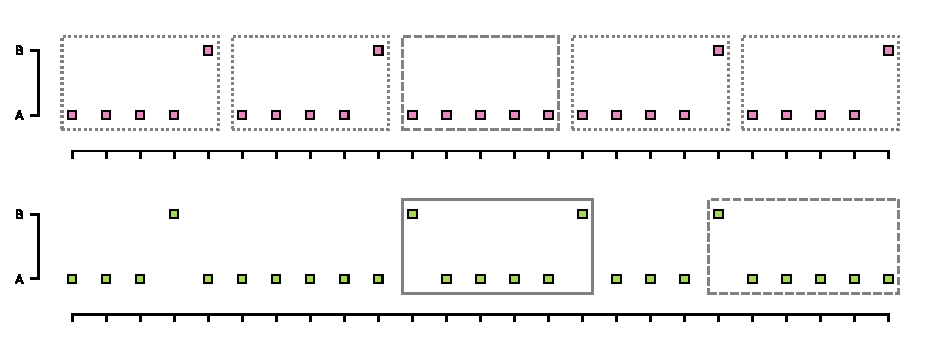
\includegraphics{figures/fig_tones.pdf}
\caption{Tones of two different frequencies (A=440 Hz, B=449 Hz) were
presented in two blocked conditions: In the \enquote{predictable}
condition (top half), tones followed a simple pattern in which a single
B-tone followed four A-tones. Some designated B-tones were replaced by
A-tones (\enquote{pattern deviants}). In the \enquote{random} condition
(lower half), tones were presented in a pseudo-random fashion ()}
\end{figure}

Participants where seated in a comfortable chair in a sound-insulated
cabin. The experimental setup was practically the same as the one used
ny Sussman, but instead of reading a book, subjects were asked to focus
their attention on a previously selected movie. Movies were presented
with subtitles but without sound. Commercially available software
(MATLAB R2014a; The MathWorks Inc, Natick, MA) in conjunction with the
Psychophysics Toolbox extension (version 3.0.12,
\textbf{brainardPsychophysicsToolbox1997?};
\textbf{kleinerWhatNewPsychtoolbox32007?}) was used to control stimulus
presentation. Stimuli consisted of pure sinusoidal tones with a duration
of 50 ms (including a 10 ms cosine on/off ramp), presented isochronously
at a stimulation onsets asynchrony (SOA) of 100 ms for study 1 and 150
ms for study 2. Overall, a total of 40 blocks containing a mixture of
frequent 440 Hz tones (\enquote{A} tones) and infrequent 449 Hz tones
(\enquote{B} tones) were delivered binaurally using Sennheiser HD-25-1
II headphones. In one half of the blocks, tones were presented in
pseudo-random order (e.g.~A-A-A-B-A-B-A\}, \enquote{random} condition),
while in the remaining block tone presentation followed a simple pattern
in which a five-tone-sequence of four frequent tones and one infrequent
tone (i.e.~A-A-A-A-B) was repeated cyclically (\enquote{predictable}
condition). Block order was counterbalanced accross participants. The
ratio of frequent and infrequent tones was 10\% for both conditions.
Within the predictable condition, 10\% of designated (infrequent) B
tones were replaced by A tones, resulting in sporadic five-tone
sequences consisting solely of A tones (i.e.~A-A-A-A-A), thus violating
the predictability rule. To assure comparability of local histories
between tones in both conditions, randomly arranged tones were
interspersed with sequences mimicking aforementioned patterns from the
predictable condition (B-A-A-A-A-B and B-A-A-A-A-A) in the random
condition. A grand total of 2000 tones in study 1 and 4000 tones in
study 2 were delivered to each participant.

\hypertarget{data-acquisition-1}{%
\subsubsection{Data Acquisition}\label{data-acquisition-1}}

Electrophysiological data was recorded from active
silver-silver-chloride (\emph{Ag}-\emph{AgCl}) electrodes using an
ActiveTwo amplifier system (BioSemi B.V., Amsterdam, The Netherlands).
Acquisition was monitored online to ensure optimal data quality. A total
of 39 channels were obtained using a 32-electrode-cap and 7 external
electrodes. Scalp electrode locations conformed to the international
10--20 system. Horizontal and vertical eye movement was obtained using
two bipolar configurations with electrodes placed around the lateral
canthi of the eyes and above and below the right eye. Additionally,
electrodes were placed on the tip of the nose and at the left and right
mastoid sites. Data was sampled at 512 Hz and on-line filtered at 1000
Hz.

\hypertarget{analysis-pipeline}{%
\subsection{Analysis Pipeline}\label{analysis-pipeline}}

Data prepossessing was implemented using a custom pipeline based on the
\emph{MNE Python} software package (Gramfort, 2013) using \emph{Python
3.7}. All computations were carried out on a cluster operated by the
University Computation Center of the University of Leipzig. Code used in
thesis is publicly available at
\url{https://github.com/marcpabst/xmas-oddballmatch}.

First, EEG data was subjected to the ZapLine procedure (de Cheveigné,
2020) to remove line noise contamination. A fivefold detection procedure
as described by Bigdely-Shamlo et al. (2015) was then used to detect and
subsequently interpolate bad channels. This specifically included the
detection of channels thain contain prolonged segments with verry small
values (i.e.~flat channels), the exclusion of channels based on robust
standard deviation (deviation criterion), unusualy pronounced
high-frequency noise (noisiness criterion), and the removal of channels
that were poorly predicted by nearby channels (correlation criterion and
predictability criterion). Channels considered bad by one or more of
these methods were removed and interpolated using spherical splines
(Perrin et al., 1989). Electrode locations for interpolations were
informed by the BESA Spherical Head Model.

For independant component anaylsis (ICA), a 1-Hz-high-pass filter (134th
order hamming-windowed FIR) was applied prior to ICA (Winkler et al.,
2015). To further reduce artifacts, Artifact Subspace Reconstruction
(ASR, Mullen et al., 2015) was used to identify and remove parts of the
data with unusual characteristics (bursts). ICA was then carried out
using the \emph{Picard} algorithm (Ablin et al., 2018, 2017) on
PCA-whitened data. To avoid rank-deficiency when extracting components
from data with one or more interpolated channels, PCA was also used for
dimensionality reduction. The EEGLAB (version 2020.0, Delorme \& Makeig,
2004) software package and the IClabel plugin (version 1.2.6,
Pion-Tonachini et al., 2019) were used to automatically classify
estimated components. Only components clearly classified
(i.e.~confidence above 50\%) as resulting from either eye movement,
muscular, or heartbeat activity were zeroed-out before applying the
mixing matrix to unfiltered data.

In line with recommendations from Widmann et al. (2015) and de Cheveigné
\& Nelken (2019), a ORDER finite impulse response (FIR) bandpass filter
from 0.1 Hz to 40 Hz (Hamming window, 0.1 Hz lower bandwith, 4 Hz upper
bandwidth, 0.0194 passband ripple, and 53 dB stopband attenuation).
Continuous data was epoched into 400 ms long segments around stimulus
onsets. Epochs included a 100 ms pre-stimulus interval. No baseline
correction was applied. Segments exeeding a peak-to-peak voltage
difference of 100 µV were removed. On average, NN epochs No data set
meet the pre-registrated exclusion criterion stated of less than 100
trials per condition, thus data from all participants (20 for 100 ms
presentation rate and 23 for 150 ms presentation rate) was analysed.

\hypertarget{statistical-analysis}{%
\subsection{Statistical Analysis}\label{statistical-analysis}}

The dependent variable for analysing missmatch response was calculated
by averaging amplitudes in a time window extedning ±25 ms around the
maximum negativity obtained by subtracting the mean ERP timecourse
following the (expected) deviant event from the ERP following the
(expected) standard event. To obtain mean amplitudes, ERPs to 4th
position A tones (A-A-A-\textbf{A}-X, \textbf{boldface} indicates the
tone of interest) and B tones (A-A-A-A-\textbf{B}) were averaged
seperatly for both the \emph{random} and the \emph{predictable}
\emph{condition}. For the \emph{random condition}, only tones that were
part of a sequence matching the patterns in the \emph{predictable}
condition were included.

In accordance with the original analysis by E. S. Sussman \& Gumenyuk
(2005), mean amplitudes for frontocentral electrodes (FZ, F3, F4, FC1,
and FC2) and the two mastoid positions (M1 and M2) were averaged
separately. Then, for both SOAs, independant three-way repeated measures
analyses of variance with factors \emph{condition} (factors
\emph{predcitable} and \emph{random}), \emph{stimulus type} (factors
\emph{A tone} and \emph{B tone}), \emph{electrode locations} (levels
\emph{fronto-central} and \emph{mastoids}), and all possible
interactions were calculated. Following this, significant interactions
effects were further investigated using post-hoc \emph{t}-tests.

Finally, the relationship between epoch number and the reliability
analysis was analyzed by drawing random subsamples of different sizes
from both our data sets and calculating split-half reliability employing
the Spearman-Brown approach. For this, single trial responses for all A
and B tones in the predictable condition were randomly shuffled. Then,
\(100, 200, ..., N_{max}\)
(\(N_{max, 100ms} = 3000, N_{max, 150ms}=1500\)) epoches were drawn,
randomly assigned to one of two halfes, and afterwards averaged
seperatly for bothtone types. Then, split-half realibility was
calculated using the differences between A and B tones in the MMN
latency window using the Sprearman-Brown prophecy formula\footnote{as
  given by \({\rho}_{xx'} = \frac{2{\rho}_{12}}{1+{\rho}_{12}}\), where
  \({\rho_{12}}\) is the Pearson correlation coefficient between the two
  halfes.} (\textbf{brownEXPERIMENTALRESULTSCORRELATION1910?};
\textbf{spearmanCorrelationCalculatedFaulty1910?}). This procedure was
repeated 100 times for each \(N\) and split-half-relaibilites thus
obtained were subsequently averaged.

\newpage

\hypertarget{results}{%
\section{Results}\label{results}}

\begin{figure}
\hypertarget{fig:fronto}{%
\centering
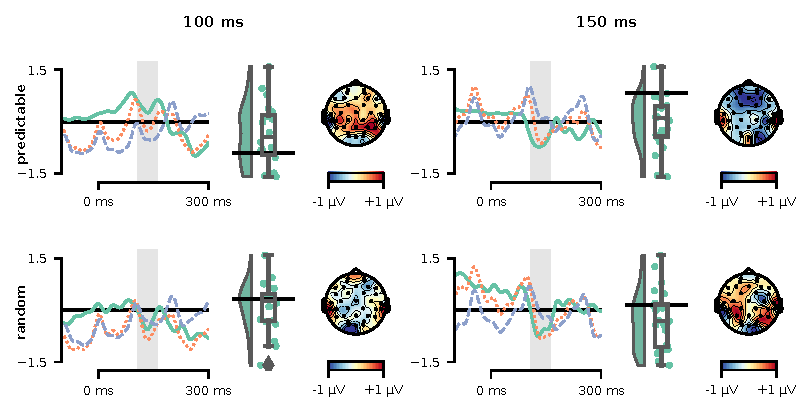
\includegraphics{figures/fig_fronto.pdf}
\caption{ERP grand averages (pooled FZ, F3, F4, FC1, and FC2 electrode
locations) for an SOA of 100 ms (left) and 150 ms (right), for A tones
(A-A-A-\textbf{A}-X, blue dashed lines) and B tones (A-A-A-A-\textbf{B},
orange dashed line) and their difference (B - A, green solid line).
Upper panels show ERPs for tones presented in a predcitable pattern
(\emph{predcitable condition}) while lower panels show ERPs for tones
presented in pseudo-random order (\emph{random condition}). Shaded area
marks MMN latency window (110 ms to 160 ms) used to calculate the
distribution of amplitude differences across particpants (middle of each
panel) and the difference of topographic maps averaged over the same
interval (right of each panel).}\label{fig:fronto}
}
\end{figure}

Grand averages of event-related potentials (ERP) at pooled FZ, F3, F4,
FC1, and FC2 electrode locations to A tones (A-A-A-\textbf{A}-X), B
tones (A-A-A-A-\textbf{B}), and their difference (\textbf{B} tone minus
\textbf{A} tone) are displayed in fig.~\ref{fig:fronto} for both 100 ms
(left panel) and 150 ms (right panel) stimulus onset asynchronies. The
top half of each panel shows ERPs in the \emph{predictable condition}
while the lower half depicts ERPs in the \emph{random condition}. For
both presentation rates, clear rhythms matching the presentation
frequency of 10 Hz (100 ms) and respectively 6.667 Hz (150 ms) are seen
as a result of substantial overlap of neighbouring tones. Panels also
show the distribution of mean amplitude differences in the MMN latency
window (as defined above, 110 ms to 160 ms after stimulus onset) across
participants and the difference of scalp topographies averaged over the
same interval. Similarly, waveforms and mean amplitude difference
distributions at pooled mastoid sites are shown in
fig.~\ref{fig:mastoids}.

\begin{figure}
\hypertarget{fig:mastoids}{%
\centering
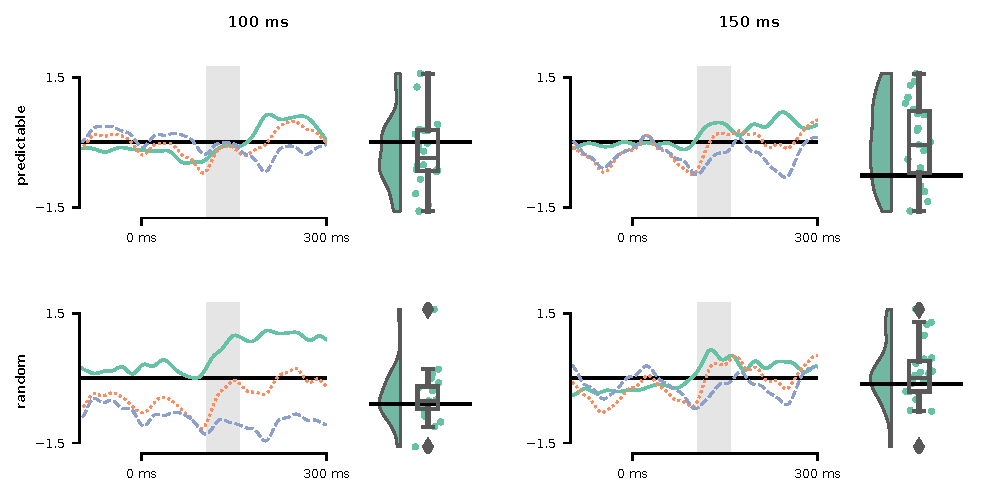
\includegraphics{figures/fig_mastoids.pdf}
\caption{ERP grand averages (pooled M1, M2 electrode locations) for an
SOA of 100 ms (left) and 150 ms (right), for A tones
(A-A-A-\textbf{A}-X, blue dashed lines) and B tones (A-A-A-A-\textbf{B},
orange dashed line) and their difference (B - A, green solid line).
Upper panels show ERPs for tones presented in a predcitable pattern
(\emph{predcitable condition}) while lower panels show ERPs for tones
presented in pseudo-random order (\emph{random condition}). Shaded area
marks MMN latency window (110 ms to 160 ms) used to calculate the
distribution of amplitude differences across
particpants.}\label{fig:mastoids}
}
\end{figure}

Evoked responses to A and B tones were compared by calculating mean
amplitudes in the MMN latency window. Mean amplitudes in the MMN latency
window and their standard deviations (SD) for all conditions are shown
in Table X. Descriptively, mean amplitudes at pooled fronto-central
electrode locations were more negative for randomly presented B tones
than for randomly presented A tones, regardless of tone presentation
rate (100 ms: \(\Delta M = -0.358 \: \mu V\); 150 ms:
\(\Delta M = -0.555 \: \mu V\)) This also held for tones presented
predictably, but for the slower of the two presentation rates only
(\(\Delta M = -0.582 \: \mu V\))). In contrast, when predictable tone
patterns occurred at a faster 100 ms rate, B tones elicited
descriptively more positive responses than A tones
(\(\Delta M = 0.383 \: \mu V\)). Descriptive comparison of evoked
responses from pooled left and right mastoids revealed that
pseudo-randomly presented B tones were more positive in the MMN latency
window than A tones (100-ms-SOA: \(\Delta M = 0.746 \: \mu V\),
150-ms-SOA: \(\Delta M = 0.510 \: \mu V\)). A similar observation could
be made for predictable B tones compared to the preceding A tones at an
SOA of 150 ms (\(\Delta M = 0.399 \: \mu V\))) but not for the faster
presentation rate (\(\Delta M = -0.132 \: \mu V\)).


  \providecommand{\huxb}[2]{\arrayrulecolor[RGB]{#1}\global\arrayrulewidth=#2pt}
  \providecommand{\huxvb}[2]{\color[RGB]{#1}\vrule width #2pt}
  \providecommand{\huxtpad}[1]{\rule{0pt}{#1}}
  \providecommand{\huxbpad}[1]{\rule[-#1]{0pt}{#1}}

\begin{table}[ht]
\begin{centerbox}
\begin{threeparttable}
 \setlength{\tabcolsep}{0pt}
\begin{tabular}{l l l l l l l}


\hhline{>{\huxb{0, 0, 0}{0.4}}->{\huxb{0, 0, 0}{0.4}}->{\huxb{0, 0, 0}{0.4}}->{\huxb{0, 0, 0}{0.4}}->{\huxb{0, 0, 0}{0.4}}->{\huxb{0, 0, 0}{0.4}}->{\huxb{0, 0, 0}{0.4}}-}
\arrayrulecolor{black}

\multicolumn{1}{!{\huxvb{0, 0, 0}{0}}l!{\huxvb{0, 0, 0}{0}}}{\huxtpad{6pt + 1em}\raggedright \hspace{0pt} \textbf{SOA} \hspace{6pt}\huxbpad{6pt}} &
\multicolumn{1}{l!{\huxvb{0, 0, 0}{0}}}{\huxtpad{6pt + 1em}\raggedright \hspace{6pt} \textbf{Condition} \hspace{6pt}\huxbpad{6pt}} &
\multicolumn{1}{l!{\huxvb{0, 0, 0}{0}}}{\huxtpad{6pt + 1em}\raggedright \hspace{6pt} \textbf{StimulusType} \hspace{6pt}\huxbpad{6pt}} &
\multicolumn{1}{r!{\huxvb{0, 0, 0}{0}}}{\huxtpad{6pt + 1em}\raggedleft \hspace{6pt} \textbf{Mean} \hspace{6pt}\huxbpad{6pt}} &
\multicolumn{1}{r!{\huxvb{0, 0, 0}{0}}}{\huxtpad{6pt + 1em}\raggedleft \hspace{6pt} \textbf{SD} \hspace{0pt}\huxbpad{6pt}} &
\multicolumn{1}{r!{\huxvb{0, 0, 0}{0}}}{\huxtpad{6pt + 1em}\raggedleft \hspace{0pt} \textbf{Mean} \hspace{6pt}\huxbpad{6pt}} &
\multicolumn{1}{r!{\huxvb{0, 0, 0}{0}}}{\huxtpad{6pt + 1em}\raggedleft \hspace{6pt} \textbf{SD} \hspace{0pt}\huxbpad{6pt}} \tabularnewline[-0.5pt]


\hhline{>{\huxb{0, 0, 0}{0.4}}->{\huxb{0, 0, 0}{0.4}}->{\huxb{0, 0, 0}{0.4}}->{\huxb{0, 0, 0}{0.4}}->{\huxb{0, 0, 0}{0.4}}->{\huxb{0, 0, 0}{0.4}}->{\huxb{0, 0, 0}{0.4}}-}
\arrayrulecolor{black}

\multicolumn{1}{!{\huxvb{0, 0, 0}{0}}l!{\huxvb{0, 0, 0}{0}}}{} &
\multicolumn{1}{l!{\huxvb{0, 0, 0}{0}}}{} &
\multicolumn{1}{l!{\huxvb{0, 0, 0}{0}}}{\huxtpad{6pt + 1em}\raggedright \hspace{6pt} A \hspace{6pt}\huxbpad{6pt}} &
\multicolumn{1}{r!{\huxvb{0, 0, 0}{0}}}{\huxtpad{6pt + 1em}\raggedleft \hspace{6pt} -0.431~ \hspace{6pt}\huxbpad{6pt}} &
\multicolumn{1}{r!{\huxvb{0, 0, 0}{0}}}{\huxtpad{6pt + 1em}\raggedleft \hspace{6pt} 1.23~ \hspace{0pt}\huxbpad{6pt}} &
\multicolumn{1}{r!{\huxvb{0, 0, 0}{0}}}{\huxtpad{6pt + 1em}\raggedleft \hspace{0pt} -0.052~ \hspace{6pt}\huxbpad{6pt}} &
\multicolumn{1}{r!{\huxvb{0, 0, 0}{0}}}{\huxtpad{6pt + 1em}\raggedleft \hspace{6pt} 1.51 \hspace{0pt}\huxbpad{6pt}} \tabularnewline[-0.5pt]


\hhline{}
\arrayrulecolor{black}

\multicolumn{1}{!{\huxvb{0, 0, 0}{0}}l!{\huxvb{0, 0, 0}{0}}}{} &
\multicolumn{1}{l!{\huxvb{0, 0, 0}{0}}}{\multirow[t]{-2}{*}[0ex]{\huxtpad{6pt + 1em}\raggedright \hspace{6pt} predictable \hspace{6pt}\huxbpad{6pt}}} &
\multicolumn{1}{l!{\huxvb{0, 0, 0}{0}}}{\huxtpad{6pt + 1em}\raggedright \hspace{6pt} B \hspace{6pt}\huxbpad{6pt}} &
\multicolumn{1}{r!{\huxvb{0, 0, 0}{0}}}{\huxtpad{6pt + 1em}\raggedleft \hspace{6pt} -0.0477 \hspace{6pt}\huxbpad{6pt}} &
\multicolumn{1}{r!{\huxvb{0, 0, 0}{0}}}{\huxtpad{6pt + 1em}\raggedleft \hspace{6pt} 1.22~ \hspace{0pt}\huxbpad{6pt}} &
\multicolumn{1}{r!{\huxvb{0, 0, 0}{0}}}{\huxtpad{6pt + 1em}\raggedleft \hspace{0pt} -0.184~ \hspace{6pt}\huxbpad{6pt}} &
\multicolumn{1}{r!{\huxvb{0, 0, 0}{0}}}{\huxtpad{6pt + 1em}\raggedleft \hspace{6pt} 1.56 \hspace{0pt}\huxbpad{6pt}} \tabularnewline[-0.5pt]


\hhline{}
\arrayrulecolor{black}

\multicolumn{1}{!{\huxvb{0, 0, 0}{0}}l!{\huxvb{0, 0, 0}{0}}}{} &
\multicolumn{1}{l!{\huxvb{0, 0, 0}{0}}}{} &
\multicolumn{1}{l!{\huxvb{0, 0, 0}{0}}}{\huxtpad{6pt + 1em}\raggedright \hspace{6pt} A \hspace{6pt}\huxbpad{6pt}} &
\multicolumn{1}{r!{\huxvb{0, 0, 0}{0}}}{\huxtpad{6pt + 1em}\raggedleft \hspace{6pt} -0.225~ \hspace{6pt}\huxbpad{6pt}} &
\multicolumn{1}{r!{\huxvb{0, 0, 0}{0}}}{\huxtpad{6pt + 1em}\raggedleft \hspace{6pt} 1.82~ \hspace{0pt}\huxbpad{6pt}} &
\multicolumn{1}{r!{\huxvb{0, 0, 0}{0}}}{\huxtpad{6pt + 1em}\raggedleft \hspace{0pt} -1.04~~ \hspace{6pt}\huxbpad{6pt}} &
\multicolumn{1}{r!{\huxvb{0, 0, 0}{0}}}{\huxtpad{6pt + 1em}\raggedleft \hspace{6pt} 2.64 \hspace{0pt}\huxbpad{6pt}} \tabularnewline[-0.5pt]


\hhline{}
\arrayrulecolor{black}

\multicolumn{1}{!{\huxvb{0, 0, 0}{0}}l!{\huxvb{0, 0, 0}{0}}}{\multirow[t]{-4}{*}[0ex]{\huxtpad{6pt + 1em}\raggedright \hspace{0pt} 100 \hspace{6pt}\huxbpad{6pt}}} &
\multicolumn{1}{l!{\huxvb{0, 0, 0}{0}}}{\multirow[t]{-2}{*}[0ex]{\huxtpad{6pt + 1em}\raggedright \hspace{6pt} random \hspace{6pt}\huxbpad{6pt}}} &
\multicolumn{1}{l!{\huxvb{0, 0, 0}{0}}}{\huxtpad{6pt + 1em}\raggedright \hspace{6pt} B \hspace{6pt}\huxbpad{6pt}} &
\multicolumn{1}{r!{\huxvb{0, 0, 0}{0}}}{\huxtpad{6pt + 1em}\raggedleft \hspace{6pt} -0.583~ \hspace{6pt}\huxbpad{6pt}} &
\multicolumn{1}{r!{\huxvb{0, 0, 0}{0}}}{\huxtpad{6pt + 1em}\raggedleft \hspace{6pt} 2.16~ \hspace{0pt}\huxbpad{6pt}} &
\multicolumn{1}{r!{\huxvb{0, 0, 0}{0}}}{\huxtpad{6pt + 1em}\raggedleft \hspace{0pt} -0.296~ \hspace{6pt}\huxbpad{6pt}} &
\multicolumn{1}{r!{\huxvb{0, 0, 0}{0}}}{\huxtpad{6pt + 1em}\raggedleft \hspace{6pt} 3.23 \hspace{0pt}\huxbpad{6pt}} \tabularnewline[-0.5pt]


\hhline{}
\arrayrulecolor{black}

\multicolumn{1}{!{\huxvb{0, 0, 0}{0}}l!{\huxvb{0, 0, 0}{0}}}{} &
\multicolumn{1}{l!{\huxvb{0, 0, 0}{0}}}{} &
\multicolumn{1}{l!{\huxvb{0, 0, 0}{0}}}{\huxtpad{6pt + 1em}\raggedright \hspace{6pt} A \hspace{6pt}\huxbpad{6pt}} &
\multicolumn{1}{r!{\huxvb{0, 0, 0}{0}}}{\huxtpad{6pt + 1em}\raggedleft \hspace{6pt} 0.25~~ \hspace{6pt}\huxbpad{6pt}} &
\multicolumn{1}{r!{\huxvb{0, 0, 0}{0}}}{\huxtpad{6pt + 1em}\raggedleft \hspace{6pt} 0.967 \hspace{0pt}\huxbpad{6pt}} &
\multicolumn{1}{r!{\huxvb{0, 0, 0}{0}}}{\huxtpad{6pt + 1em}\raggedleft \hspace{0pt} -0.349~ \hspace{6pt}\huxbpad{6pt}} &
\multicolumn{1}{r!{\huxvb{0, 0, 0}{0}}}{\huxtpad{6pt + 1em}\raggedleft \hspace{6pt} 1.19 \hspace{0pt}\huxbpad{6pt}} \tabularnewline[-0.5pt]


\hhline{}
\arrayrulecolor{black}

\multicolumn{1}{!{\huxvb{0, 0, 0}{0}}l!{\huxvb{0, 0, 0}{0}}}{} &
\multicolumn{1}{l!{\huxvb{0, 0, 0}{0}}}{\multirow[t]{-2}{*}[0ex]{\huxtpad{6pt + 1em}\raggedright \hspace{6pt} predictable \hspace{6pt}\huxbpad{6pt}}} &
\multicolumn{1}{l!{\huxvb{0, 0, 0}{0}}}{\huxtpad{6pt + 1em}\raggedright \hspace{6pt} B \hspace{6pt}\huxbpad{6pt}} &
\multicolumn{1}{r!{\huxvb{0, 0, 0}{0}}}{\huxtpad{6pt + 1em}\raggedleft \hspace{6pt} -0.331~ \hspace{6pt}\huxbpad{6pt}} &
\multicolumn{1}{r!{\huxvb{0, 0, 0}{0}}}{\huxtpad{6pt + 1em}\raggedleft \hspace{6pt} 1.09~ \hspace{0pt}\huxbpad{6pt}} &
\multicolumn{1}{r!{\huxvb{0, 0, 0}{0}}}{\huxtpad{6pt + 1em}\raggedleft \hspace{0pt} 0.0492 \hspace{6pt}\huxbpad{6pt}} &
\multicolumn{1}{r!{\huxvb{0, 0, 0}{0}}}{\huxtpad{6pt + 1em}\raggedleft \hspace{6pt} 1.33 \hspace{0pt}\huxbpad{6pt}} \tabularnewline[-0.5pt]


\hhline{}
\arrayrulecolor{black}

\multicolumn{1}{!{\huxvb{0, 0, 0}{0}}l!{\huxvb{0, 0, 0}{0}}}{} &
\multicolumn{1}{l!{\huxvb{0, 0, 0}{0}}}{} &
\multicolumn{1}{l!{\huxvb{0, 0, 0}{0}}}{\huxtpad{6pt + 1em}\raggedright \hspace{6pt} A \hspace{6pt}\huxbpad{6pt}} &
\multicolumn{1}{r!{\huxvb{0, 0, 0}{0}}}{\huxtpad{6pt + 1em}\raggedleft \hspace{6pt} 0.0233 \hspace{6pt}\huxbpad{6pt}} &
\multicolumn{1}{r!{\huxvb{0, 0, 0}{0}}}{\huxtpad{6pt + 1em}\raggedleft \hspace{6pt} 1.75~ \hspace{0pt}\huxbpad{6pt}} &
\multicolumn{1}{r!{\huxvb{0, 0, 0}{0}}}{\huxtpad{6pt + 1em}\raggedleft \hspace{0pt} -0.292~ \hspace{6pt}\huxbpad{6pt}} &
\multicolumn{1}{r!{\huxvb{0, 0, 0}{0}}}{\huxtpad{6pt + 1em}\raggedleft \hspace{6pt} 1.64 \hspace{0pt}\huxbpad{6pt}} \tabularnewline[-0.5pt]


\hhline{}
\arrayrulecolor{black}

\multicolumn{1}{!{\huxvb{0, 0, 0}{0}}l!{\huxvb{0, 0, 0}{0}}}{\multirow[t]{-4}{*}[0ex]{\huxtpad{6pt + 1em}\raggedright \hspace{0pt} 150 \hspace{6pt}\huxbpad{6pt}}} &
\multicolumn{1}{l!{\huxvb{0, 0, 0}{0}}}{\multirow[t]{-2}{*}[0ex]{\huxtpad{6pt + 1em}\raggedright \hspace{6pt} random \hspace{6pt}\huxbpad{6pt}}} &
\multicolumn{1}{l!{\huxvb{0, 0, 0}{0}}}{\huxtpad{6pt + 1em}\raggedright \hspace{6pt} B \hspace{6pt}\huxbpad{6pt}} &
\multicolumn{1}{r!{\huxvb{0, 0, 0}{0}}}{\huxtpad{6pt + 1em}\raggedleft \hspace{6pt} -0.531~ \hspace{6pt}\huxbpad{6pt}} &
\multicolumn{1}{r!{\huxvb{0, 0, 0}{0}}}{\huxtpad{6pt + 1em}\raggedleft \hspace{6pt} 1.82~ \hspace{0pt}\huxbpad{6pt}} &
\multicolumn{1}{r!{\huxvb{0, 0, 0}{0}}}{\huxtpad{6pt + 1em}\raggedleft \hspace{0pt} 0.218~ \hspace{6pt}\huxbpad{6pt}} &
\multicolumn{1}{r!{\huxvb{0, 0, 0}{0}}}{\huxtpad{6pt + 1em}\raggedleft \hspace{6pt} 2.38 \hspace{0pt}\huxbpad{6pt}} \tabularnewline[-0.5pt]


\hhline{>{\huxb{0, 0, 0}{0.4}}->{\huxb{0, 0, 0}{0.4}}->{\huxb{0, 0, 0}{0.4}}->{\huxb{0, 0, 0}{0.4}}->{\huxb{0, 0, 0}{0.4}}->{\huxb{0, 0, 0}{0.4}}->{\huxb{0, 0, 0}{0.4}}-}
\arrayrulecolor{black}
\end{tabular}
\end{threeparttable}\par\end{centerbox}

\end{table}



Inference statistics provided support for these findings. For the 100 ms
stimulation rate, the three-way ANOVA yielded a significant three-way
interaction effect (\emph{condition} x \emph{stimulus type} x
\emph{electrode locations}; \(F(1,19) = 7.53\), \(p = .013\)) but failed
to reveal main effects for factors \emph{stimulus type}
(\(F(1,19) = 1.05\), \(p = .318\)), \emph{condition}
(\(F(1,19) = 0.83\), \(p = .373\)), and \emph{electrode locations}
(\(F(1,19) = 0.04\), \(p = .852\)). In contrast, for tones presented at
a SOA of 150 ms only the two-way interaction term \emph{stimulus type} x
\emph{electrode locations} had a significant effect
(\(F(1,22) = 20.76\), \(p = 0.0002\)). Mean amplitudes in the MMN
latency window however did not differ for factors \emph{stimulus type}
(\(F(1,22) = 0.32\), \(p = 0.5790\)), \emph{electrode locations}
(\(F(1,22) = 0.04\), \(p = 0.8540\)) or \emph{condition}
(\(F(1,22) = 0.08\), \(p = 0.7800\)).


  \providecommand{\huxb}[2]{\arrayrulecolor[RGB]{#1}\global\arrayrulewidth=#2pt}
  \providecommand{\huxvb}[2]{\color[RGB]{#1}\vrule width #2pt}
  \providecommand{\huxtpad}[1]{\rule{0pt}{#1}}
  \providecommand{\huxbpad}[1]{\rule[-#1]{0pt}{#1}}

\begin{table}[ht]
\begin{centerbox}
\begin{threeparttable}
\captionsetup{justification=centering,singlelinecheck=off}
\caption{Results of the 3-way ANOVA (condition x stimulus x electrode) for repeated measures conducted on the mean ERP-amplitudes (time window 111 - 161 ms) at electrode Fz (upper section). The significant interaction between the three factors included was further analyzed by 2-way ANOVAS (stimulus x electrode) conducted separately for the random condition (middle section) and the predictable condition (lower section).}
 \setlength{\tabcolsep}{0pt}
\begin{tabular}{l l l l l l l l}


\hhline{>{\huxb{0, 0, 0}{0.4}}->{\huxb{0, 0, 0}{0.4}}->{\huxb{0, 0, 0}{0.4}}->{\huxb{0, 0, 0}{0.4}}->{\huxb{0, 0, 0}{0.4}}->{\huxb{0, 0, 0}{0.4}}->{\huxb{0, 0, 0}{0.4}}->{\huxb{0, 0, 0}{0.4}}-}
\arrayrulecolor{black}

\multicolumn{1}{!{\huxvb{0, 0, 0}{0}}l!{\huxvb{0, 0, 0}{0}}}{\huxtpad{6pt + 1em}\raggedright \hspace{0pt} \rotatebox{90}{\textbf{}} \hspace{6pt}\huxbpad{6pt}} &
\multicolumn{1}{l!{\huxvb{0, 0, 0}{0}}}{\huxtpad{6pt + 1em}\raggedright \hspace{6pt} \textbf{Effect} \hspace{6pt}\huxbpad{6pt}} &
\multicolumn{1}{r!{\huxvb{0, 0, 0}{0}}}{\huxtpad{6pt + 1em}\raggedleft \hspace{6pt} \textbf{DFn} \hspace{6pt}\huxbpad{6pt}} &
\multicolumn{1}{r!{\huxvb{0, 0, 0}{0}}}{\huxtpad{6pt + 1em}\raggedleft \hspace{6pt} \textbf{DFd} \hspace{6pt}\huxbpad{6pt}} &
\multicolumn{1}{r!{\huxvb{0, 0, 0}{0}}}{\huxtpad{6pt + 1em}\raggedleft \hspace{6pt} \textbf{F} \hspace{6pt}\huxbpad{6pt}} &
\multicolumn{1}{r!{\huxvb{0, 0, 0}{0}}}{\huxtpad{6pt + 1em}\raggedleft \hspace{6pt} \textbf{p} \hspace{6pt}\huxbpad{6pt}} &
\multicolumn{1}{l!{\huxvb{0, 0, 0}{0}}}{\huxtpad{6pt + 1em}\raggedright \hspace{6pt} \textbf{p$<$.05} \hspace{6pt}\huxbpad{6pt}} &
\multicolumn{1}{r!{\huxvb{0, 0, 0}{0}}}{\huxtpad{6pt + 1em}\raggedleft \hspace{6pt} \textbf{ges} \hspace{0pt}\huxbpad{6pt}} \tabularnewline[-0.5pt]


\hhline{>{\huxb{0, 0, 0}{0.4}}->{\huxb{0, 0, 0}{0.4}}->{\huxb{0, 0, 0}{0.4}}->{\huxb{0, 0, 0}{0.4}}->{\huxb{0, 0, 0}{0.4}}->{\huxb{0, 0, 0}{0.4}}->{\huxb{0, 0, 0}{0.4}}->{\huxb{0, 0, 0}{0.4}}-}
\arrayrulecolor{black}

\multicolumn{1}{!{\huxvb{0, 0, 0}{0}}l!{\huxvb{0, 0, 0}{0}}}{} &
\multicolumn{1}{l!{\huxvb{0, 0, 0}{0}}}{\huxtpad{6pt + 1em}\raggedright \hspace{6pt} Condition \hspace{6pt}\huxbpad{6pt}} &
\multicolumn{1}{r!{\huxvb{0, 0, 0}{0}}}{\huxtpad{6pt + 1em}\raggedleft \hspace{6pt} 1 \hspace{6pt}\huxbpad{6pt}} &
\multicolumn{1}{r!{\huxvb{0, 0, 0}{0}}}{\huxtpad{6pt + 1em}\raggedleft \hspace{6pt} 19 \hspace{6pt}\huxbpad{6pt}} &
\multicolumn{1}{r!{\huxvb{0, 0, 0}{0}}}{\huxtpad{6pt + 1em}\raggedleft \hspace{6pt} 0.831 \hspace{6pt}\huxbpad{6pt}} &
\multicolumn{1}{r!{\huxvb{0, 0, 0}{0}}}{\huxtpad{6pt + 1em}\raggedleft \hspace{6pt} 0.373~~~ \hspace{6pt}\huxbpad{6pt}} &
\multicolumn{1}{l!{\huxvb{0, 0, 0}{0}}}{\huxtpad{6pt + 1em}\raggedright \hspace{6pt}  \hspace{6pt}\huxbpad{6pt}} &
\multicolumn{1}{r!{\huxvb{0, 0, 0}{0}}}{\huxtpad{6pt + 1em}\raggedleft \hspace{6pt} 0.008~~~ \hspace{0pt}\huxbpad{6pt}} \tabularnewline[-0.5pt]


\hhline{}
\arrayrulecolor{black}

\multicolumn{1}{!{\huxvb{0, 0, 0}{0}}l!{\huxvb{0, 0, 0}{0}}}{} &
\multicolumn{1}{l!{\huxvb{0, 0, 0}{0}}}{\huxtpad{6pt + 1em}\raggedright \hspace{6pt} StimulusType \hspace{6pt}\huxbpad{6pt}} &
\multicolumn{1}{r!{\huxvb{0, 0, 0}{0}}}{\huxtpad{6pt + 1em}\raggedleft \hspace{6pt} 1 \hspace{6pt}\huxbpad{6pt}} &
\multicolumn{1}{r!{\huxvb{0, 0, 0}{0}}}{\huxtpad{6pt + 1em}\raggedleft \hspace{6pt} 19 \hspace{6pt}\huxbpad{6pt}} &
\multicolumn{1}{r!{\huxvb{0, 0, 0}{0}}}{\huxtpad{6pt + 1em}\raggedleft \hspace{6pt} 1.05~ \hspace{6pt}\huxbpad{6pt}} &
\multicolumn{1}{r!{\huxvb{0, 0, 0}{0}}}{\huxtpad{6pt + 1em}\raggedleft \hspace{6pt} 0.318~~~ \hspace{6pt}\huxbpad{6pt}} &
\multicolumn{1}{l!{\huxvb{0, 0, 0}{0}}}{\huxtpad{6pt + 1em}\raggedright \hspace{6pt}  \hspace{6pt}\huxbpad{6pt}} &
\multicolumn{1}{r!{\huxvb{0, 0, 0}{0}}}{\huxtpad{6pt + 1em}\raggedleft \hspace{6pt} 0.002~~~ \hspace{0pt}\huxbpad{6pt}} \tabularnewline[-0.5pt]


\hhline{}
\arrayrulecolor{black}

\multicolumn{1}{!{\huxvb{0, 0, 0}{0}}l!{\huxvb{0, 0, 0}{0}}}{} &
\multicolumn{1}{l!{\huxvb{0, 0, 0}{0}}}{\huxtpad{6pt + 1em}\raggedright \hspace{6pt} Electrode \hspace{6pt}\huxbpad{6pt}} &
\multicolumn{1}{r!{\huxvb{0, 0, 0}{0}}}{\huxtpad{6pt + 1em}\raggedleft \hspace{6pt} 1 \hspace{6pt}\huxbpad{6pt}} &
\multicolumn{1}{r!{\huxvb{0, 0, 0}{0}}}{\huxtpad{6pt + 1em}\raggedleft \hspace{6pt} 19 \hspace{6pt}\huxbpad{6pt}} &
\multicolumn{1}{r!{\huxvb{0, 0, 0}{0}}}{\huxtpad{6pt + 1em}\raggedleft \hspace{6pt} 0.036 \hspace{6pt}\huxbpad{6pt}} &
\multicolumn{1}{r!{\huxvb{0, 0, 0}{0}}}{\huxtpad{6pt + 1em}\raggedleft \hspace{6pt} 0.852~~~ \hspace{6pt}\huxbpad{6pt}} &
\multicolumn{1}{l!{\huxvb{0, 0, 0}{0}}}{\huxtpad{6pt + 1em}\raggedright \hspace{6pt}  \hspace{6pt}\huxbpad{6pt}} &
\multicolumn{1}{r!{\huxvb{0, 0, 0}{0}}}{\huxtpad{6pt + 1em}\raggedleft \hspace{6pt} 0.000331 \hspace{0pt}\huxbpad{6pt}} \tabularnewline[-0.5pt]


\hhline{}
\arrayrulecolor{black}

\multicolumn{1}{!{\huxvb{0, 0, 0}{0}}l!{\huxvb{0, 0, 0}{0}}}{} &
\multicolumn{1}{l!{\huxvb{0, 0, 0}{0}}}{\huxtpad{6pt + 1em}\raggedright \hspace{6pt} Condition x StimulusType \hspace{6pt}\huxbpad{6pt}} &
\multicolumn{1}{r!{\huxvb{0, 0, 0}{0}}}{\huxtpad{6pt + 1em}\raggedleft \hspace{6pt} 1 \hspace{6pt}\huxbpad{6pt}} &
\multicolumn{1}{r!{\huxvb{0, 0, 0}{0}}}{\huxtpad{6pt + 1em}\raggedleft \hspace{6pt} 19 \hspace{6pt}\huxbpad{6pt}} &
\multicolumn{1}{r!{\huxvb{0, 0, 0}{0}}}{\huxtpad{6pt + 1em}\raggedleft \hspace{6pt} 0.051 \hspace{6pt}\huxbpad{6pt}} &
\multicolumn{1}{r!{\huxvb{0, 0, 0}{0}}}{\huxtpad{6pt + 1em}\raggedleft \hspace{6pt} 0.823~~~ \hspace{6pt}\huxbpad{6pt}} &
\multicolumn{1}{l!{\huxvb{0, 0, 0}{0}}}{\huxtpad{6pt + 1em}\raggedright \hspace{6pt}  \hspace{6pt}\huxbpad{6pt}} &
\multicolumn{1}{r!{\huxvb{0, 0, 0}{0}}}{\huxtpad{6pt + 1em}\raggedleft \hspace{6pt} 7.55e-05 \hspace{0pt}\huxbpad{6pt}} \tabularnewline[-0.5pt]


\hhline{}
\arrayrulecolor{black}

\multicolumn{1}{!{\huxvb{0, 0, 0}{0}}l!{\huxvb{0, 0, 0}{0}}}{} &
\multicolumn{1}{l!{\huxvb{0, 0, 0}{0}}}{\huxtpad{6pt + 1em}\raggedright \hspace{6pt} Condition x Electrode \hspace{6pt}\huxbpad{6pt}} &
\multicolumn{1}{r!{\huxvb{0, 0, 0}{0}}}{\huxtpad{6pt + 1em}\raggedleft \hspace{6pt} 1 \hspace{6pt}\huxbpad{6pt}} &
\multicolumn{1}{r!{\huxvb{0, 0, 0}{0}}}{\huxtpad{6pt + 1em}\raggedleft \hspace{6pt} 19 \hspace{6pt}\huxbpad{6pt}} &
\multicolumn{1}{r!{\huxvb{0, 0, 0}{0}}}{\huxtpad{6pt + 1em}\raggedleft \hspace{6pt} 0.763 \hspace{6pt}\huxbpad{6pt}} &
\multicolumn{1}{r!{\huxvb{0, 0, 0}{0}}}{\huxtpad{6pt + 1em}\raggedleft \hspace{6pt} 0.393~~~ \hspace{6pt}\huxbpad{6pt}} &
\multicolumn{1}{l!{\huxvb{0, 0, 0}{0}}}{\huxtpad{6pt + 1em}\raggedright \hspace{6pt}  \hspace{6pt}\huxbpad{6pt}} &
\multicolumn{1}{r!{\huxvb{0, 0, 0}{0}}}{\huxtpad{6pt + 1em}\raggedleft \hspace{6pt} 0.002~~~ \hspace{0pt}\huxbpad{6pt}} \tabularnewline[-0.5pt]


\hhline{}
\arrayrulecolor{black}

\multicolumn{1}{!{\huxvb{0, 0, 0}{0}}l!{\huxvb{0, 0, 0}{0}}}{} &
\multicolumn{1}{l!{\huxvb{0, 0, 0}{0}}}{\huxtpad{6pt + 1em}\raggedright \hspace{6pt} StimulusType x Electrode \hspace{6pt}\huxbpad{6pt}} &
\multicolumn{1}{r!{\huxvb{0, 0, 0}{0}}}{\huxtpad{6pt + 1em}\raggedleft \hspace{6pt} 1 \hspace{6pt}\huxbpad{6pt}} &
\multicolumn{1}{r!{\huxvb{0, 0, 0}{0}}}{\huxtpad{6pt + 1em}\raggedleft \hspace{6pt} 19 \hspace{6pt}\huxbpad{6pt}} &
\multicolumn{1}{r!{\huxvb{0, 0, 0}{0}}}{\huxtpad{6pt + 1em}\raggedleft \hspace{6pt} 0.797 \hspace{6pt}\huxbpad{6pt}} &
\multicolumn{1}{r!{\huxvb{0, 0, 0}{0}}}{\huxtpad{6pt + 1em}\raggedleft \hspace{6pt} 0.383~~~ \hspace{6pt}\huxbpad{6pt}} &
\multicolumn{1}{l!{\huxvb{0, 0, 0}{0}}}{\huxtpad{6pt + 1em}\raggedright \hspace{6pt}  \hspace{6pt}\huxbpad{6pt}} &
\multicolumn{1}{r!{\huxvb{0, 0, 0}{0}}}{\huxtpad{6pt + 1em}\raggedleft \hspace{6pt} 0.001~~~ \hspace{0pt}\huxbpad{6pt}} \tabularnewline[-0.5pt]


\hhline{}
\arrayrulecolor{black}

\multicolumn{1}{!{\huxvb{0, 0, 0}{0}}l!{\huxvb{0, 0, 0}{0}}}{\multirow[c]{-7}{*}[0ex]{\huxtpad{6pt + 1em}\raggedright \hspace{0pt} \rotatebox{90}{100 ms} \hspace{6pt}\huxbpad{6pt}}} &
\multicolumn{1}{l!{\huxvb{0, 0, 0}{0}}}{\huxtpad{6pt + 1em}\raggedright \hspace{6pt} Condition x StimulusType x Electrode \hspace{6pt}\huxbpad{15pt}} &
\multicolumn{1}{r!{\huxvb{0, 0, 0}{0}}}{\huxtpad{6pt + 1em}\raggedleft \hspace{6pt} 1 \hspace{6pt}\huxbpad{15pt}} &
\multicolumn{1}{r!{\huxvb{0, 0, 0}{0}}}{\huxtpad{6pt + 1em}\raggedleft \hspace{6pt} 19 \hspace{6pt}\huxbpad{15pt}} &
\multicolumn{1}{r!{\huxvb{0, 0, 0}{0}}}{\huxtpad{6pt + 1em}\raggedleft \hspace{6pt} 7.53~ \hspace{6pt}\huxbpad{15pt}} &
\multicolumn{1}{r!{\huxvb{0, 0, 0}{0}}}{\huxtpad{6pt + 1em}\raggedleft \hspace{6pt} 0.013~~~ \hspace{6pt}\huxbpad{15pt}} &
\multicolumn{1}{l!{\huxvb{0, 0, 0}{0}}}{\huxtpad{6pt + 1em}\raggedright \hspace{6pt} * \hspace{6pt}\huxbpad{15pt}} &
\multicolumn{1}{r!{\huxvb{0, 0, 0}{0}}}{\huxtpad{6pt + 1em}\raggedleft \hspace{6pt} 0.01~~~~ \hspace{0pt}\huxbpad{15pt}} \tabularnewline[-0.5pt]


\hhline{}
\arrayrulecolor{black}

\multicolumn{1}{!{\huxvb{0, 0, 0}{0}}l!{\huxvb{0, 0, 0}{0}}}{} &
\multicolumn{1}{l!{\huxvb{0, 0, 0}{0}}}{\huxtpad{15pt + 1em}\raggedright \hspace{6pt} Condition \hspace{6pt}\huxbpad{6pt}} &
\multicolumn{1}{r!{\huxvb{0, 0, 0}{0}}}{\huxtpad{15pt + 1em}\raggedleft \hspace{6pt} 1 \hspace{6pt}\huxbpad{6pt}} &
\multicolumn{1}{r!{\huxvb{0, 0, 0}{0}}}{\huxtpad{15pt + 1em}\raggedleft \hspace{6pt} 22 \hspace{6pt}\huxbpad{6pt}} &
\multicolumn{1}{r!{\huxvb{0, 0, 0}{0}}}{\huxtpad{15pt + 1em}\raggedleft \hspace{6pt} 0.08~ \hspace{6pt}\huxbpad{6pt}} &
\multicolumn{1}{r!{\huxvb{0, 0, 0}{0}}}{\huxtpad{15pt + 1em}\raggedleft \hspace{6pt} 0.78~~~~ \hspace{6pt}\huxbpad{6pt}} &
\multicolumn{1}{l!{\huxvb{0, 0, 0}{0}}}{\huxtpad{15pt + 1em}\raggedright \hspace{6pt}  \hspace{6pt}\huxbpad{6pt}} &
\multicolumn{1}{r!{\huxvb{0, 0, 0}{0}}}{\huxtpad{15pt + 1em}\raggedleft \hspace{6pt} 0.000263 \hspace{0pt}\huxbpad{6pt}} \tabularnewline[-0.5pt]


\hhline{}
\arrayrulecolor{black}

\multicolumn{1}{!{\huxvb{0, 0, 0}{0}}l!{\huxvb{0, 0, 0}{0}}}{} &
\multicolumn{1}{l!{\huxvb{0, 0, 0}{0}}}{\huxtpad{6pt + 1em}\raggedright \hspace{6pt} StimulusType \hspace{6pt}\huxbpad{6pt}} &
\multicolumn{1}{r!{\huxvb{0, 0, 0}{0}}}{\huxtpad{6pt + 1em}\raggedleft \hspace{6pt} 1 \hspace{6pt}\huxbpad{6pt}} &
\multicolumn{1}{r!{\huxvb{0, 0, 0}{0}}}{\huxtpad{6pt + 1em}\raggedleft \hspace{6pt} 22 \hspace{6pt}\huxbpad{6pt}} &
\multicolumn{1}{r!{\huxvb{0, 0, 0}{0}}}{\huxtpad{6pt + 1em}\raggedleft \hspace{6pt} 0.317 \hspace{6pt}\huxbpad{6pt}} &
\multicolumn{1}{r!{\huxvb{0, 0, 0}{0}}}{\huxtpad{6pt + 1em}\raggedleft \hspace{6pt} 0.579~~~ \hspace{6pt}\huxbpad{6pt}} &
\multicolumn{1}{l!{\huxvb{0, 0, 0}{0}}}{\huxtpad{6pt + 1em}\raggedright \hspace{6pt}  \hspace{6pt}\huxbpad{6pt}} &
\multicolumn{1}{r!{\huxvb{0, 0, 0}{0}}}{\huxtpad{6pt + 1em}\raggedleft \hspace{6pt} 0.000339 \hspace{0pt}\huxbpad{6pt}} \tabularnewline[-0.5pt]


\hhline{}
\arrayrulecolor{black}

\multicolumn{1}{!{\huxvb{0, 0, 0}{0}}l!{\huxvb{0, 0, 0}{0}}}{} &
\multicolumn{1}{l!{\huxvb{0, 0, 0}{0}}}{\huxtpad{6pt + 1em}\raggedright \hspace{6pt} Electrode \hspace{6pt}\huxbpad{6pt}} &
\multicolumn{1}{r!{\huxvb{0, 0, 0}{0}}}{\huxtpad{6pt + 1em}\raggedleft \hspace{6pt} 1 \hspace{6pt}\huxbpad{6pt}} &
\multicolumn{1}{r!{\huxvb{0, 0, 0}{0}}}{\huxtpad{6pt + 1em}\raggedleft \hspace{6pt} 22 \hspace{6pt}\huxbpad{6pt}} &
\multicolumn{1}{r!{\huxvb{0, 0, 0}{0}}}{\huxtpad{6pt + 1em}\raggedleft \hspace{6pt} 0.035 \hspace{6pt}\huxbpad{6pt}} &
\multicolumn{1}{r!{\huxvb{0, 0, 0}{0}}}{\huxtpad{6pt + 1em}\raggedleft \hspace{6pt} 0.854~~~ \hspace{6pt}\huxbpad{6pt}} &
\multicolumn{1}{l!{\huxvb{0, 0, 0}{0}}}{\huxtpad{6pt + 1em}\raggedright \hspace{6pt}  \hspace{6pt}\huxbpad{6pt}} &
\multicolumn{1}{r!{\huxvb{0, 0, 0}{0}}}{\huxtpad{6pt + 1em}\raggedleft \hspace{6pt} 0.000301 \hspace{0pt}\huxbpad{6pt}} \tabularnewline[-0.5pt]


\hhline{}
\arrayrulecolor{black}

\multicolumn{1}{!{\huxvb{0, 0, 0}{0}}l!{\huxvb{0, 0, 0}{0}}}{} &
\multicolumn{1}{l!{\huxvb{0, 0, 0}{0}}}{\huxtpad{6pt + 1em}\raggedright \hspace{6pt} Condition x StimulusType \hspace{6pt}\huxbpad{6pt}} &
\multicolumn{1}{r!{\huxvb{0, 0, 0}{0}}}{\huxtpad{6pt + 1em}\raggedleft \hspace{6pt} 1 \hspace{6pt}\huxbpad{6pt}} &
\multicolumn{1}{r!{\huxvb{0, 0, 0}{0}}}{\huxtpad{6pt + 1em}\raggedleft \hspace{6pt} 22 \hspace{6pt}\huxbpad{6pt}} &
\multicolumn{1}{r!{\huxvb{0, 0, 0}{0}}}{\huxtpad{6pt + 1em}\raggedleft \hspace{6pt} 0.16~ \hspace{6pt}\huxbpad{6pt}} &
\multicolumn{1}{r!{\huxvb{0, 0, 0}{0}}}{\huxtpad{6pt + 1em}\raggedleft \hspace{6pt} 0.693~~~ \hspace{6pt}\huxbpad{6pt}} &
\multicolumn{1}{l!{\huxvb{0, 0, 0}{0}}}{\huxtpad{6pt + 1em}\raggedright \hspace{6pt}  \hspace{6pt}\huxbpad{6pt}} &
\multicolumn{1}{r!{\huxvb{0, 0, 0}{0}}}{\huxtpad{6pt + 1em}\raggedleft \hspace{6pt} 0.000124 \hspace{0pt}\huxbpad{6pt}} \tabularnewline[-0.5pt]


\hhline{}
\arrayrulecolor{black}

\multicolumn{1}{!{\huxvb{0, 0, 0}{0}}l!{\huxvb{0, 0, 0}{0}}}{} &
\multicolumn{1}{l!{\huxvb{0, 0, 0}{0}}}{\huxtpad{6pt + 1em}\raggedright \hspace{6pt} Condition x Electrode \hspace{6pt}\huxbpad{6pt}} &
\multicolumn{1}{r!{\huxvb{0, 0, 0}{0}}}{\huxtpad{6pt + 1em}\raggedleft \hspace{6pt} 1 \hspace{6pt}\huxbpad{6pt}} &
\multicolumn{1}{r!{\huxvb{0, 0, 0}{0}}}{\huxtpad{6pt + 1em}\raggedleft \hspace{6pt} 22 \hspace{6pt}\huxbpad{6pt}} &
\multicolumn{1}{r!{\huxvb{0, 0, 0}{0}}}{\huxtpad{6pt + 1em}\raggedleft \hspace{6pt} 1.13~ \hspace{6pt}\huxbpad{6pt}} &
\multicolumn{1}{r!{\huxvb{0, 0, 0}{0}}}{\huxtpad{6pt + 1em}\raggedleft \hspace{6pt} 0.299~~~ \hspace{6pt}\huxbpad{6pt}} &
\multicolumn{1}{l!{\huxvb{0, 0, 0}{0}}}{\huxtpad{6pt + 1em}\raggedright \hspace{6pt}  \hspace{6pt}\huxbpad{6pt}} &
\multicolumn{1}{r!{\huxvb{0, 0, 0}{0}}}{\huxtpad{6pt + 1em}\raggedleft \hspace{6pt} 0.003~~~ \hspace{0pt}\huxbpad{6pt}} \tabularnewline[-0.5pt]


\hhline{}
\arrayrulecolor{black}

\multicolumn{1}{!{\huxvb{0, 0, 0}{0}}l!{\huxvb{0, 0, 0}{0}}}{} &
\multicolumn{1}{l!{\huxvb{0, 0, 0}{0}}}{\huxtpad{6pt + 1em}\raggedright \hspace{6pt} StimulusType x Electrode \hspace{6pt}\huxbpad{6pt}} &
\multicolumn{1}{r!{\huxvb{0, 0, 0}{0}}}{\huxtpad{6pt + 1em}\raggedleft \hspace{6pt} 1 \hspace{6pt}\huxbpad{6pt}} &
\multicolumn{1}{r!{\huxvb{0, 0, 0}{0}}}{\huxtpad{6pt + 1em}\raggedleft \hspace{6pt} 22 \hspace{6pt}\huxbpad{6pt}} &
\multicolumn{1}{r!{\huxvb{0, 0, 0}{0}}}{\huxtpad{6pt + 1em}\raggedleft \hspace{6pt} 20.8~~ \hspace{6pt}\huxbpad{6pt}} &
\multicolumn{1}{r!{\huxvb{0, 0, 0}{0}}}{\huxtpad{6pt + 1em}\raggedleft \hspace{6pt} 0.000155 \hspace{6pt}\huxbpad{6pt}} &
\multicolumn{1}{l!{\huxvb{0, 0, 0}{0}}}{\huxtpad{6pt + 1em}\raggedright \hspace{6pt} * \hspace{6pt}\huxbpad{6pt}} &
\multicolumn{1}{r!{\huxvb{0, 0, 0}{0}}}{\huxtpad{6pt + 1em}\raggedleft \hspace{6pt} 0.026~~~ \hspace{0pt}\huxbpad{6pt}} \tabularnewline[-0.5pt]


\hhline{}
\arrayrulecolor{black}

\multicolumn{1}{!{\huxvb{0, 0, 0}{0}}l!{\huxvb{0, 0, 0}{0}}}{\multirow[c]{-7}{*}[0ex]{\huxtpad{15pt + 1em}\raggedright \hspace{0pt} \rotatebox{90}{150 ms} \hspace{6pt}\huxbpad{6pt}}} &
\multicolumn{1}{l!{\huxvb{0, 0, 0}{0}}}{\huxtpad{6pt + 1em}\raggedright \hspace{6pt} Condition x StimulusType x Electrode \hspace{6pt}\huxbpad{6pt}} &
\multicolumn{1}{r!{\huxvb{0, 0, 0}{0}}}{\huxtpad{6pt + 1em}\raggedleft \hspace{6pt} 1 \hspace{6pt}\huxbpad{6pt}} &
\multicolumn{1}{r!{\huxvb{0, 0, 0}{0}}}{\huxtpad{6pt + 1em}\raggedleft \hspace{6pt} 22 \hspace{6pt}\huxbpad{6pt}} &
\multicolumn{1}{r!{\huxvb{0, 0, 0}{0}}}{\huxtpad{6pt + 1em}\raggedleft \hspace{6pt} 0.053 \hspace{6pt}\huxbpad{6pt}} &
\multicolumn{1}{r!{\huxvb{0, 0, 0}{0}}}{\huxtpad{6pt + 1em}\raggedleft \hspace{6pt} 0.819~~~ \hspace{6pt}\huxbpad{6pt}} &
\multicolumn{1}{l!{\huxvb{0, 0, 0}{0}}}{\huxtpad{6pt + 1em}\raggedright \hspace{6pt}  \hspace{6pt}\huxbpad{6pt}} &
\multicolumn{1}{r!{\huxvb{0, 0, 0}{0}}}{\huxtpad{6pt + 1em}\raggedleft \hspace{6pt} 4.63e-05 \hspace{0pt}\huxbpad{6pt}} \tabularnewline[-0.5pt]


\hhline{>{\huxb{0, 0, 0}{0.4}}->{\huxb{0, 0, 0}{0.4}}->{\huxb{0, 0, 0}{0.4}}->{\huxb{0, 0, 0}{0.4}}->{\huxb{0, 0, 0}{0.4}}->{\huxb{0, 0, 0}{0.4}}->{\huxb{0, 0, 0}{0.4}}->{\huxb{0, 0, 0}{0.4}}-}
\arrayrulecolor{black}
\end{tabular}
\end{threeparttable}\par\end{centerbox}

\end{table}



Two-way ANOVAs (\emph{condition} x \emph{stimulus type}) were carried
out separately for pooled fronto-central and mastoid electrode
locations. For 100 ms tone presentation rate, the \emph{condition} x
\emph{stimulus type} interaction only resulted in a significant effect
for the fronto-central electrode cluster (\(F(1,19) = 16.75\),
\(p = 0.0006\)) but not for pooled mastoid sites (\(F(1,19) = 2.37\),
\(p = 0.1410\)) indicating that the three-way interaction effect
\emph{condition} x \emph{stimulus type} x \emph{electrode} is indeed
driven by the amplitude differences in the fronto-central electrode
locations . Contrary to this, for the 150 ms presentation rate, main
effects for \emph{stimulus type} were significant for both
fronto-central and mastoid sites, suggesting that there was both an MMN
at fronto-central locations as well as a polarity-reversal at the
mastoid electrodes.


  \providecommand{\huxb}[2]{\arrayrulecolor[RGB]{#1}\global\arrayrulewidth=#2pt}
  \providecommand{\huxvb}[2]{\color[RGB]{#1}\vrule width #2pt}
  \providecommand{\huxtpad}[1]{\rule{0pt}{#1}}
  \providecommand{\huxbpad}[1]{\rule[-#1]{0pt}{#1}}

\begin{table}[ht]
\begin{centerbox}
\begin{threeparttable}
\captionsetup{justification=centering,singlelinecheck=off}
\caption{Results of the 2-way ANOVA (condition x stimulus type) for repeated measures. Only fronto included.}
 \setlength{\tabcolsep}{0pt}
\begin{tabular}{l l l l l l l l l}


\hhline{>{\huxb{0, 0, 0}{0.4}}->{\huxb{0, 0, 0}{0.4}}->{\huxb{0, 0, 0}{0.4}}->{\huxb{0, 0, 0}{0.4}}->{\huxb{0, 0, 0}{0.4}}->{\huxb{0, 0, 0}{0.4}}->{\huxb{0, 0, 0}{0.4}}->{\huxb{0, 0, 0}{0.4}}->{\huxb{0, 0, 0}{0.4}}-}
\arrayrulecolor{black}

\multicolumn{1}{!{\huxvb{0, 0, 0}{0}}l!{\huxvb{0, 0, 0}{0}}}{\huxtpad{6pt + 1em}\raggedright \hspace{0pt} \rotatebox{90}{\textbf{}} \hspace{6pt}\huxbpad{6pt}} &
\multicolumn{1}{l!{\huxvb{0, 0, 0}{0}}}{\huxtpad{6pt + 1em}\raggedright \hspace{6pt} \rotatebox{90}{\textbf{}} \hspace{6pt}\huxbpad{6pt}} &
\multicolumn{1}{l!{\huxvb{0, 0, 0}{0}}}{\huxtpad{6pt + 1em}\raggedright \hspace{6pt} \textbf{Effect} \hspace{6pt}\huxbpad{6pt}} &
\multicolumn{1}{r!{\huxvb{0, 0, 0}{0}}}{\huxtpad{6pt + 1em}\raggedleft \hspace{6pt} \textbf{DFn} \hspace{6pt}\huxbpad{6pt}} &
\multicolumn{1}{r!{\huxvb{0, 0, 0}{0}}}{\huxtpad{6pt + 1em}\raggedleft \hspace{6pt} \textbf{DFd} \hspace{6pt}\huxbpad{6pt}} &
\multicolumn{1}{r!{\huxvb{0, 0, 0}{0}}}{\huxtpad{6pt + 1em}\raggedleft \hspace{6pt} \textbf{F} \hspace{6pt}\huxbpad{6pt}} &
\multicolumn{1}{r!{\huxvb{0, 0, 0}{0}}}{\huxtpad{6pt + 1em}\raggedleft \hspace{6pt} \textbf{p} \hspace{6pt}\huxbpad{6pt}} &
\multicolumn{1}{l!{\huxvb{0, 0, 0}{0}}}{\huxtpad{6pt + 1em}\raggedright \hspace{6pt} \textbf{p$<$.05} \hspace{6pt}\huxbpad{6pt}} &
\multicolumn{1}{r!{\huxvb{0, 0, 0}{0}}}{\huxtpad{6pt + 1em}\raggedleft \hspace{6pt} \textbf{ges} \hspace{0pt}\huxbpad{6pt}} \tabularnewline[-0.5pt]


\hhline{>{\huxb{0, 0, 0}{0.4}}->{\huxb{0, 0, 0}{0.4}}->{\huxb{0, 0, 0}{0.4}}->{\huxb{0, 0, 0}{0.4}}->{\huxb{0, 0, 0}{0.4}}->{\huxb{0, 0, 0}{0.4}}->{\huxb{0, 0, 0}{0.4}}->{\huxb{0, 0, 0}{0.4}}->{\huxb{0, 0, 0}{0.4}}-}
\arrayrulecolor{black}

\multicolumn{1}{!{\huxvb{0, 0, 0}{0}}l!{\huxvb{0, 0, 0}{0}}}{} &
\multicolumn{1}{l!{\huxvb{0, 0, 0}{0}}}{} &
\multicolumn{1}{l!{\huxvb{0, 0, 0}{0}}}{\huxtpad{6pt + 1em}\raggedright \hspace{6pt} Condition \hspace{6pt}\huxbpad{6pt}} &
\multicolumn{1}{r!{\huxvb{0, 0, 0}{0}}}{\huxtpad{6pt + 1em}\raggedleft \hspace{6pt} 1 \hspace{6pt}\huxbpad{6pt}} &
\multicolumn{1}{r!{\huxvb{0, 0, 0}{0}}}{\huxtpad{6pt + 1em}\raggedleft \hspace{6pt} 19 \hspace{6pt}\huxbpad{6pt}} &
\multicolumn{1}{r!{\huxvb{0, 0, 0}{0}}}{\huxtpad{6pt + 1em}\raggedleft \hspace{6pt} 0.137 \hspace{6pt}\huxbpad{6pt}} &
\multicolumn{1}{r!{\huxvb{0, 0, 0}{0}}}{\huxtpad{6pt + 1em}\raggedleft \hspace{6pt} .715 \hspace{6pt}\huxbpad{6pt}} &
\multicolumn{1}{l!{\huxvb{0, 0, 0}{0}}}{\huxtpad{6pt + 1em}\raggedright \hspace{6pt}  \hspace{6pt}\huxbpad{6pt}} &
\multicolumn{1}{r!{\huxvb{0, 0, 0}{0}}}{\huxtpad{6pt + 1em}\raggedleft \hspace{6pt} 0.002~~~ \hspace{0pt}\huxbpad{6pt}} \tabularnewline[-0.5pt]


\hhline{}
\arrayrulecolor{black}

\multicolumn{1}{!{\huxvb{0, 0, 0}{0}}l!{\huxvb{0, 0, 0}{0}}}{} &
\multicolumn{1}{l!{\huxvb{0, 0, 0}{0}}}{} &
\multicolumn{1}{l!{\huxvb{0, 0, 0}{0}}}{\huxtpad{6pt + 1em}\raggedright \hspace{6pt} StimulusType \hspace{6pt}\huxbpad{6pt}} &
\multicolumn{1}{r!{\huxvb{0, 0, 0}{0}}}{\huxtpad{6pt + 1em}\raggedleft \hspace{6pt} 1 \hspace{6pt}\huxbpad{6pt}} &
\multicolumn{1}{r!{\huxvb{0, 0, 0}{0}}}{\huxtpad{6pt + 1em}\raggedleft \hspace{6pt} 19 \hspace{6pt}\huxbpad{6pt}} &
\multicolumn{1}{r!{\huxvb{0, 0, 0}{0}}}{\huxtpad{6pt + 1em}\raggedleft \hspace{6pt} 0.004 \hspace{6pt}\huxbpad{6pt}} &
\multicolumn{1}{r!{\huxvb{0, 0, 0}{0}}}{\huxtpad{6pt + 1em}\raggedleft \hspace{6pt} .953 \hspace{6pt}\huxbpad{6pt}} &
\multicolumn{1}{l!{\huxvb{0, 0, 0}{0}}}{\huxtpad{6pt + 1em}\raggedright \hspace{6pt}  \hspace{6pt}\huxbpad{6pt}} &
\multicolumn{1}{r!{\huxvb{0, 0, 0}{0}}}{\huxtpad{6pt + 1em}\raggedleft \hspace{6pt} 8.21e-06 \hspace{0pt}\huxbpad{6pt}} \tabularnewline[-0.5pt]


\hhline{}
\arrayrulecolor{black}

\multicolumn{1}{!{\huxvb{0, 0, 0}{0}}l!{\huxvb{0, 0, 0}{0}}}{} &
\multicolumn{1}{l!{\huxvb{0, 0, 0}{0}}}{\multirow[c]{-3}{*}[0ex]{\huxtpad{6pt + 1em}\raggedright \hspace{6pt} \rotatebox{90}{Frontal} \hspace{6pt}\huxbpad{6pt}}} &
\multicolumn{1}{l!{\huxvb{0, 0, 0}{0}}}{\huxtpad{6pt + 1em}\raggedright \hspace{6pt} Condition x StimulusType \hspace{6pt}\huxbpad{8pt}} &
\multicolumn{1}{r!{\huxvb{0, 0, 0}{0}}}{\huxtpad{6pt + 1em}\raggedleft \hspace{6pt} 1 \hspace{6pt}\huxbpad{8pt}} &
\multicolumn{1}{r!{\huxvb{0, 0, 0}{0}}}{\huxtpad{6pt + 1em}\raggedleft \hspace{6pt} 19 \hspace{6pt}\huxbpad{8pt}} &
\multicolumn{1}{r!{\huxvb{0, 0, 0}{0}}}{\huxtpad{6pt + 1em}\raggedleft \hspace{6pt} 17~~~~ \hspace{6pt}\huxbpad{8pt}} &
\multicolumn{1}{r!{\huxvb{0, 0, 0}{0}}}{\huxtpad{6pt + 1em}\raggedleft \hspace{6pt} $<$ .001 \hspace{6pt}\huxbpad{8pt}} &
\multicolumn{1}{l!{\huxvb{0, 0, 0}{0}}}{\huxtpad{6pt + 1em}\raggedright \hspace{6pt} * \hspace{6pt}\huxbpad{8pt}} &
\multicolumn{1}{r!{\huxvb{0, 0, 0}{0}}}{\huxtpad{6pt + 1em}\raggedleft \hspace{6pt} 0.013~~~ \hspace{0pt}\huxbpad{8pt}} \tabularnewline[-0.5pt]


\hhline{}
\arrayrulecolor{black}

\multicolumn{1}{!{\huxvb{0, 0, 0}{0}}l!{\huxvb{0, 0, 0}{0}}}{} &
\multicolumn{1}{l!{\huxvb{0, 0, 0}{0}}}{} &
\multicolumn{1}{l!{\huxvb{0, 0, 0}{0}}}{\huxtpad{8pt + 1em}\raggedright \hspace{6pt} Condition \hspace{6pt}\huxbpad{6pt}} &
\multicolumn{1}{r!{\huxvb{0, 0, 0}{0}}}{\huxtpad{8pt + 1em}\raggedleft \hspace{6pt} 1 \hspace{6pt}\huxbpad{6pt}} &
\multicolumn{1}{r!{\huxvb{0, 0, 0}{0}}}{\huxtpad{8pt + 1em}\raggedleft \hspace{6pt} 19 \hspace{6pt}\huxbpad{6pt}} &
\multicolumn{1}{r!{\huxvb{0, 0, 0}{0}}}{\huxtpad{8pt + 1em}\raggedleft \hspace{6pt} 1.39~ \hspace{6pt}\huxbpad{6pt}} &
\multicolumn{1}{r!{\huxvb{0, 0, 0}{0}}}{\huxtpad{8pt + 1em}\raggedleft \hspace{6pt} .253 \hspace{6pt}\huxbpad{6pt}} &
\multicolumn{1}{l!{\huxvb{0, 0, 0}{0}}}{\huxtpad{8pt + 1em}\raggedright \hspace{6pt}  \hspace{6pt}\huxbpad{6pt}} &
\multicolumn{1}{r!{\huxvb{0, 0, 0}{0}}}{\huxtpad{8pt + 1em}\raggedleft \hspace{6pt} 0.015~~~ \hspace{0pt}\huxbpad{6pt}} \tabularnewline[-0.5pt]


\hhline{}
\arrayrulecolor{black}

\multicolumn{1}{!{\huxvb{0, 0, 0}{0}}l!{\huxvb{0, 0, 0}{0}}}{} &
\multicolumn{1}{l!{\huxvb{0, 0, 0}{0}}}{} &
\multicolumn{1}{l!{\huxvb{0, 0, 0}{0}}}{\huxtpad{6pt + 1em}\raggedright \hspace{6pt} StimulusType \hspace{6pt}\huxbpad{6pt}} &
\multicolumn{1}{r!{\huxvb{0, 0, 0}{0}}}{\huxtpad{6pt + 1em}\raggedleft \hspace{6pt} 1 \hspace{6pt}\huxbpad{6pt}} &
\multicolumn{1}{r!{\huxvb{0, 0, 0}{0}}}{\huxtpad{6pt + 1em}\raggedleft \hspace{6pt} 19 \hspace{6pt}\huxbpad{6pt}} &
\multicolumn{1}{r!{\huxvb{0, 0, 0}{0}}}{\huxtpad{6pt + 1em}\raggedleft \hspace{6pt} 0.946 \hspace{6pt}\huxbpad{6pt}} &
\multicolumn{1}{r!{\huxvb{0, 0, 0}{0}}}{\huxtpad{6pt + 1em}\raggedleft \hspace{6pt} .343 \hspace{6pt}\huxbpad{6pt}} &
\multicolumn{1}{l!{\huxvb{0, 0, 0}{0}}}{\huxtpad{6pt + 1em}\raggedright \hspace{6pt}  \hspace{6pt}\huxbpad{6pt}} &
\multicolumn{1}{r!{\huxvb{0, 0, 0}{0}}}{\huxtpad{6pt + 1em}\raggedleft \hspace{6pt} 0.003~~~ \hspace{0pt}\huxbpad{6pt}} \tabularnewline[-0.5pt]


\hhline{}
\arrayrulecolor{black}

\multicolumn{1}{!{\huxvb{0, 0, 0}{0}}l!{\huxvb{0, 0, 0}{0}}}{\multirow[c]{-6}{*}[0ex]{\huxtpad{6pt + 1em}\raggedright \hspace{0pt} \rotatebox{90}{100 ms} \hspace{6pt}\huxbpad{6pt}}} &
\multicolumn{1}{l!{\huxvb{0, 0, 0}{0}}}{\multirow[c]{-3}{*}[0ex]{\huxtpad{8pt + 1em}\raggedright \hspace{6pt} \rotatebox{90}{Mastoids} \hspace{6pt}\huxbpad{6pt}}} &
\multicolumn{1}{l!{\huxvb{0, 0, 0}{0}}}{\huxtpad{6pt + 1em}\raggedright \hspace{6pt} Condition x StimulusType \hspace{6pt}\huxbpad{15pt}} &
\multicolumn{1}{r!{\huxvb{0, 0, 0}{0}}}{\huxtpad{6pt + 1em}\raggedleft \hspace{6pt} 1 \hspace{6pt}\huxbpad{15pt}} &
\multicolumn{1}{r!{\huxvb{0, 0, 0}{0}}}{\huxtpad{6pt + 1em}\raggedleft \hspace{6pt} 19 \hspace{6pt}\huxbpad{15pt}} &
\multicolumn{1}{r!{\huxvb{0, 0, 0}{0}}}{\huxtpad{6pt + 1em}\raggedleft \hspace{6pt} 2.2~~ \hspace{6pt}\huxbpad{15pt}} &
\multicolumn{1}{r!{\huxvb{0, 0, 0}{0}}}{\huxtpad{6pt + 1em}\raggedleft \hspace{6pt} .154 \hspace{6pt}\huxbpad{15pt}} &
\multicolumn{1}{l!{\huxvb{0, 0, 0}{0}}}{\huxtpad{6pt + 1em}\raggedright \hspace{6pt}  \hspace{6pt}\huxbpad{15pt}} &
\multicolumn{1}{r!{\huxvb{0, 0, 0}{0}}}{\huxtpad{6pt + 1em}\raggedleft \hspace{6pt} 0.008~~~ \hspace{0pt}\huxbpad{15pt}} \tabularnewline[-0.5pt]


\hhline{}
\arrayrulecolor{black}

\multicolumn{1}{!{\huxvb{0, 0, 0}{0}}l!{\huxvb{0, 0, 0}{0}}}{} &
\multicolumn{1}{l!{\huxvb{0, 0, 0}{0}}}{} &
\multicolumn{1}{l!{\huxvb{0, 0, 0}{0}}}{\huxtpad{15pt + 1em}\raggedright \hspace{6pt} Condition \hspace{6pt}\huxbpad{6pt}} &
\multicolumn{1}{r!{\huxvb{0, 0, 0}{0}}}{\huxtpad{15pt + 1em}\raggedleft \hspace{6pt} 1 \hspace{6pt}\huxbpad{6pt}} &
\multicolumn{1}{r!{\huxvb{0, 0, 0}{0}}}{\huxtpad{15pt + 1em}\raggedleft \hspace{6pt} 22 \hspace{6pt}\huxbpad{6pt}} &
\multicolumn{1}{r!{\huxvb{0, 0, 0}{0}}}{\huxtpad{15pt + 1em}\raggedleft \hspace{6pt} 0.775 \hspace{6pt}\huxbpad{6pt}} &
\multicolumn{1}{r!{\huxvb{0, 0, 0}{0}}}{\huxtpad{15pt + 1em}\raggedleft \hspace{6pt} .388 \hspace{6pt}\huxbpad{6pt}} &
\multicolumn{1}{l!{\huxvb{0, 0, 0}{0}}}{\huxtpad{15pt + 1em}\raggedright \hspace{6pt}  \hspace{6pt}\huxbpad{6pt}} &
\multicolumn{1}{r!{\huxvb{0, 0, 0}{0}}}{\huxtpad{15pt + 1em}\raggedleft \hspace{6pt} 0.005~~~ \hspace{0pt}\huxbpad{6pt}} \tabularnewline[-0.5pt]


\hhline{}
\arrayrulecolor{black}

\multicolumn{1}{!{\huxvb{0, 0, 0}{0}}l!{\huxvb{0, 0, 0}{0}}}{} &
\multicolumn{1}{l!{\huxvb{0, 0, 0}{0}}}{} &
\multicolumn{1}{l!{\huxvb{0, 0, 0}{0}}}{\huxtpad{6pt + 1em}\raggedright \hspace{6pt} StimulusType \hspace{6pt}\huxbpad{6pt}} &
\multicolumn{1}{r!{\huxvb{0, 0, 0}{0}}}{\huxtpad{6pt + 1em}\raggedleft \hspace{6pt} 1 \hspace{6pt}\huxbpad{6pt}} &
\multicolumn{1}{r!{\huxvb{0, 0, 0}{0}}}{\huxtpad{6pt + 1em}\raggedleft \hspace{6pt} 22 \hspace{6pt}\huxbpad{6pt}} &
\multicolumn{1}{r!{\huxvb{0, 0, 0}{0}}}{\huxtpad{6pt + 1em}\raggedleft \hspace{6pt} 21.6~~ \hspace{6pt}\huxbpad{6pt}} &
\multicolumn{1}{r!{\huxvb{0, 0, 0}{0}}}{\huxtpad{6pt + 1em}\raggedleft \hspace{6pt} $<$ .001 \hspace{6pt}\huxbpad{6pt}} &
\multicolumn{1}{l!{\huxvb{0, 0, 0}{0}}}{\huxtpad{6pt + 1em}\raggedright \hspace{6pt} * \hspace{6pt}\huxbpad{6pt}} &
\multicolumn{1}{r!{\huxvb{0, 0, 0}{0}}}{\huxtpad{6pt + 1em}\raggedleft \hspace{6pt} 0.036~~~ \hspace{0pt}\huxbpad{6pt}} \tabularnewline[-0.5pt]


\hhline{}
\arrayrulecolor{black}

\multicolumn{1}{!{\huxvb{0, 0, 0}{0}}l!{\huxvb{0, 0, 0}{0}}}{} &
\multicolumn{1}{l!{\huxvb{0, 0, 0}{0}}}{\multirow[c]{-3}{*}[0ex]{\huxtpad{15pt + 1em}\raggedright \hspace{6pt} \rotatebox{90}{Frontal} \hspace{6pt}\huxbpad{6pt}}} &
\multicolumn{1}{l!{\huxvb{0, 0, 0}{0}}}{\huxtpad{6pt + 1em}\raggedright \hspace{6pt} Condition x StimulusType \hspace{6pt}\huxbpad{8pt}} &
\multicolumn{1}{r!{\huxvb{0, 0, 0}{0}}}{\huxtpad{6pt + 1em}\raggedleft \hspace{6pt} 1 \hspace{6pt}\huxbpad{8pt}} &
\multicolumn{1}{r!{\huxvb{0, 0, 0}{0}}}{\huxtpad{6pt + 1em}\raggedleft \hspace{6pt} 22 \hspace{6pt}\huxbpad{8pt}} &
\multicolumn{1}{r!{\huxvb{0, 0, 0}{0}}}{\huxtpad{6pt + 1em}\raggedleft \hspace{6pt} 0.194 \hspace{6pt}\huxbpad{8pt}} &
\multicolumn{1}{r!{\huxvb{0, 0, 0}{0}}}{\huxtpad{6pt + 1em}\raggedleft \hspace{6pt} .664 \hspace{6pt}\huxbpad{8pt}} &
\multicolumn{1}{l!{\huxvb{0, 0, 0}{0}}}{\huxtpad{6pt + 1em}\raggedright \hspace{6pt}  \hspace{6pt}\huxbpad{8pt}} &
\multicolumn{1}{r!{\huxvb{0, 0, 0}{0}}}{\huxtpad{6pt + 1em}\raggedleft \hspace{6pt} 0.000147 \hspace{0pt}\huxbpad{8pt}} \tabularnewline[-0.5pt]


\hhline{}
\arrayrulecolor{black}

\multicolumn{1}{!{\huxvb{0, 0, 0}{0}}l!{\huxvb{0, 0, 0}{0}}}{} &
\multicolumn{1}{l!{\huxvb{0, 0, 0}{0}}}{} &
\multicolumn{1}{l!{\huxvb{0, 0, 0}{0}}}{\huxtpad{8pt + 1em}\raggedright \hspace{6pt} Condition \hspace{6pt}\huxbpad{6pt}} &
\multicolumn{1}{r!{\huxvb{0, 0, 0}{0}}}{\huxtpad{8pt + 1em}\raggedleft \hspace{6pt} 1 \hspace{6pt}\huxbpad{6pt}} &
\multicolumn{1}{r!{\huxvb{0, 0, 0}{0}}}{\huxtpad{8pt + 1em}\raggedleft \hspace{6pt} 22 \hspace{6pt}\huxbpad{6pt}} &
\multicolumn{1}{r!{\huxvb{0, 0, 0}{0}}}{\huxtpad{8pt + 1em}\raggedleft \hspace{6pt} 0.187 \hspace{6pt}\huxbpad{6pt}} &
\multicolumn{1}{r!{\huxvb{0, 0, 0}{0}}}{\huxtpad{8pt + 1em}\raggedleft \hspace{6pt} .670 \hspace{6pt}\huxbpad{6pt}} &
\multicolumn{1}{l!{\huxvb{0, 0, 0}{0}}}{\huxtpad{8pt + 1em}\raggedright \hspace{6pt}  \hspace{6pt}\huxbpad{6pt}} &
\multicolumn{1}{r!{\huxvb{0, 0, 0}{0}}}{\huxtpad{8pt + 1em}\raggedleft \hspace{6pt} 0.001~~~ \hspace{0pt}\huxbpad{6pt}} \tabularnewline[-0.5pt]


\hhline{}
\arrayrulecolor{black}

\multicolumn{1}{!{\huxvb{0, 0, 0}{0}}l!{\huxvb{0, 0, 0}{0}}}{} &
\multicolumn{1}{l!{\huxvb{0, 0, 0}{0}}}{} &
\multicolumn{1}{l!{\huxvb{0, 0, 0}{0}}}{\huxtpad{6pt + 1em}\raggedright \hspace{6pt} StimulusType \hspace{6pt}\huxbpad{6pt}} &
\multicolumn{1}{r!{\huxvb{0, 0, 0}{0}}}{\huxtpad{6pt + 1em}\raggedleft \hspace{6pt} 1 \hspace{6pt}\huxbpad{6pt}} &
\multicolumn{1}{r!{\huxvb{0, 0, 0}{0}}}{\huxtpad{6pt + 1em}\raggedleft \hspace{6pt} 22 \hspace{6pt}\huxbpad{6pt}} &
\multicolumn{1}{r!{\huxvb{0, 0, 0}{0}}}{\huxtpad{6pt + 1em}\raggedleft \hspace{6pt} 6.26~ \hspace{6pt}\huxbpad{6pt}} &
\multicolumn{1}{r!{\huxvb{0, 0, 0}{0}}}{\huxtpad{6pt + 1em}\raggedleft \hspace{6pt} .020 \hspace{6pt}\huxbpad{6pt}} &
\multicolumn{1}{l!{\huxvb{0, 0, 0}{0}}}{\huxtpad{6pt + 1em}\raggedright \hspace{6pt} * \hspace{6pt}\huxbpad{6pt}} &
\multicolumn{1}{r!{\huxvb{0, 0, 0}{0}}}{\huxtpad{6pt + 1em}\raggedleft \hspace{6pt} 0.017~~~ \hspace{0pt}\huxbpad{6pt}} \tabularnewline[-0.5pt]


\hhline{}
\arrayrulecolor{black}

\multicolumn{1}{!{\huxvb{0, 0, 0}{0}}l!{\huxvb{0, 0, 0}{0}}}{\multirow[c]{-6}{*}[0ex]{\huxtpad{15pt + 1em}\raggedright \hspace{0pt} \rotatebox{90}{150 ms} \hspace{6pt}\huxbpad{6pt}}} &
\multicolumn{1}{l!{\huxvb{0, 0, 0}{0}}}{\multirow[c]{-3}{*}[0ex]{\huxtpad{8pt + 1em}\raggedright \hspace{6pt} \rotatebox{90}{Mastoids} \hspace{6pt}\huxbpad{6pt}}} &
\multicolumn{1}{l!{\huxvb{0, 0, 0}{0}}}{\huxtpad{6pt + 1em}\raggedright \hspace{6pt} Condition x StimulusType \hspace{6pt}\huxbpad{6pt}} &
\multicolumn{1}{r!{\huxvb{0, 0, 0}{0}}}{\huxtpad{6pt + 1em}\raggedleft \hspace{6pt} 1 \hspace{6pt}\huxbpad{6pt}} &
\multicolumn{1}{r!{\huxvb{0, 0, 0}{0}}}{\huxtpad{6pt + 1em}\raggedleft \hspace{6pt} 22 \hspace{6pt}\huxbpad{6pt}} &
\multicolumn{1}{r!{\huxvb{0, 0, 0}{0}}}{\huxtpad{6pt + 1em}\raggedleft \hspace{6pt} 0.102 \hspace{6pt}\huxbpad{6pt}} &
\multicolumn{1}{r!{\huxvb{0, 0, 0}{0}}}{\huxtpad{6pt + 1em}\raggedleft \hspace{6pt} .753 \hspace{6pt}\huxbpad{6pt}} &
\multicolumn{1}{l!{\huxvb{0, 0, 0}{0}}}{\huxtpad{6pt + 1em}\raggedright \hspace{6pt}  \hspace{6pt}\huxbpad{6pt}} &
\multicolumn{1}{r!{\huxvb{0, 0, 0}{0}}}{\huxtpad{6pt + 1em}\raggedleft \hspace{6pt} 0.000236 \hspace{0pt}\huxbpad{6pt}} \tabularnewline[-0.5pt]


\hhline{>{\huxb{0, 0, 0}{0.4}}->{\huxb{0, 0, 0}{0.4}}->{\huxb{0, 0, 0}{0.4}}->{\huxb{0, 0, 0}{0.4}}->{\huxb{0, 0, 0}{0.4}}->{\huxb{0, 0, 0}{0.4}}->{\huxb{0, 0, 0}{0.4}}->{\huxb{0, 0, 0}{0.4}}->{\huxb{0, 0, 0}{0.4}}-}
\arrayrulecolor{black}
\end{tabular}
\end{threeparttable}\par\end{centerbox}

\end{table}



Post-hoc tests between ERPs to A and B tones were carried out using
two-tailed Student's \emph{t}-tests over the differnce. P-values were
corrected for multiple comparisons using the Benjamini--Hochberg step-up
procedure. For the 100 ms SOA, results indicated a significant effect
only for predictable tones at fronto-central electrodes
(\(t(19) = -2.77\), \(p = .025\), \(CI_{.95} = [-0.67,-0.09]\)). For the
150 ms SOA, B tones elicited significantly more negative ERPs than B
tones at fronto-central electrode locations in both predictable
(\(t(22) = 5.20\), \(p < .001\), \(CI_{.95} = [0.35,0.81]\)) and random
(\(t(22) = 3.28\), \(p = .009\), \(CI_{.95} = [0.20,0.91]\)) conditions.
Significant polarity reversal effects at mastoid sites were only present
for predictable (\(t(22) = -3.95\), \(p = .003\),
\(CI_{.95} = [-0.61,-0.19]\)) tones but not for randomly presented
(\(t(22) = -1.59\), \(p = .169\), \(CI_{.95} = [-1.18,0.16]\)) tones.

\begin{figure}
\centering
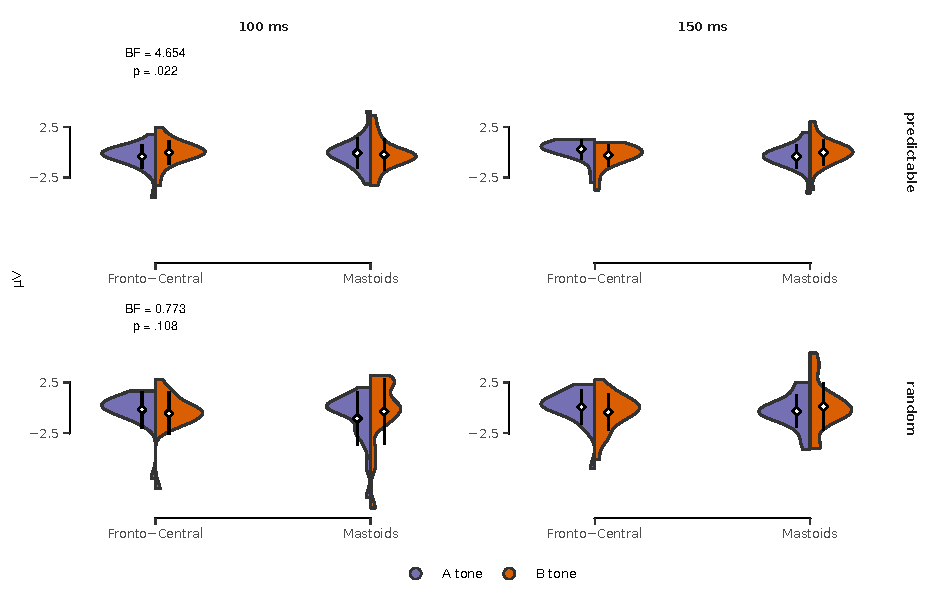
\includegraphics{figures/fig_posthoc.pdf}
\caption{Averaged voltages in the MMN latency window for pooled
fronto-central and mastoid electrodes. Colored areas show sample
probability density function for A tones (green) and B tones (red).
White diamonds indicate estimated population mean, vertical bars
represent 95\%-conficence interval. Only Benjamini-Hochberg-corrected
p-values \(< 0.05\) are shown.}
\end{figure}

Fig.~\ref{fig:sequences} shows EEG waveform averages for five-tone
sequences (A-A-A-A-B) presented in a \emph{predictable} (top panel) and
\emph{random} contexts (lower panel).

\begin{figure}
\hypertarget{fig:rel}{%
\centering
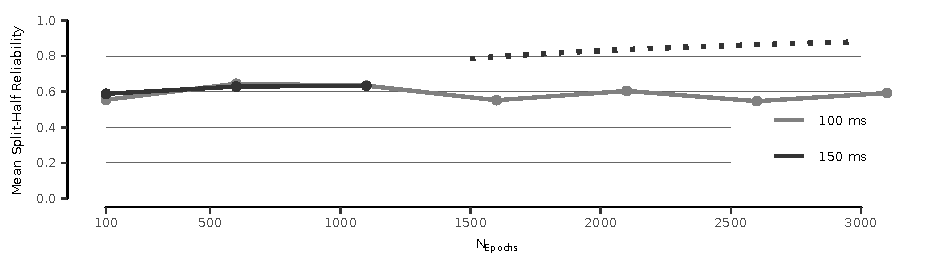
\includegraphics{figures/fig_subsample_rel.pdf}
\caption{EEG waveforms for five-tone sequences presented in an
predictable context (dotted line) and pseudo-random condition (dashed
line) for 100 ms presentation rate (top panel) and 150 ms presentation
rate (lower pabel). Vertical lines indicate tone onset.}\label{fig:rel}
}
\end{figure}

Split-half reliabilities are displayed in fig.~\ref{fig:rel}. Simulated
values match the curve expected from the Spearman-Brown formula. In the
context of classcial test theory, this method relates the length of a
test (or \emph{experiment}) to the number of items (or \emph{trials}).
The first derivitve of the Spearman-Brown function is monotonically
decreasing, leading to two different observation: i) Adding additional
epochs (extending the test length by an absolute value in classcial test
theory terms) has a large effect when the number of already present
epochs is low, but has only little effect when already dealing with
large numbers of epochs and ii) SOA and thus effect sized have a larger
impact when epoch numbers are small compared to high epoch numbers.
Graphed values also show that reliabilities for the 100 ms stimulation
rate are considerably lower than for an SOA of 150 ms and that
reliabilities are very low when using a relatively small number of
epochs. There is no generally accepted rule as to the level above which
the coefficient can be considered acceptable. Rather, reliabiliy should
be evaluated based on the purpose of a study considering the
cost-benefit trade-off (\textbf{nunnallyPsychometricTheory1994?}). As
laid out, inreased realibility comes at overproportionate cost, in that
collecting more samples will not increase ralibility by the same factor.
That said, many published articles deem reliability coefficients above
.7 or .8 \enquote{acceptable} (\textbf{lanceSourcesFourCommonly2006?}).

\begin{figure}
\hypertarget{fig:sequences}{%
\centering
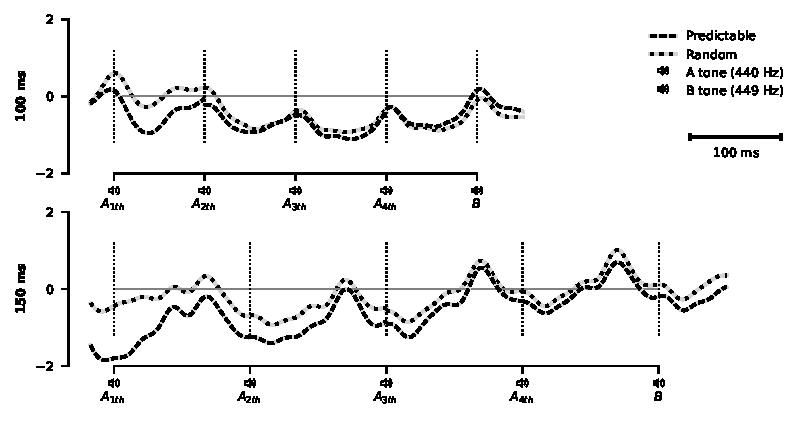
\includegraphics{figures/fig_sequences.pdf}
\caption{EEG waveforms for five-tone sequences presented in an
predictable context (dotted line) and pseudo-random condition (dashed
line) for 100 ms presentation rate (top panel) and 150 ms presentation
rate (lower pabel). Vertical lines indicate tone
onset.}\label{fig:sequences}
}
\end{figure}

Lorem ipsum dolor sit amet, consectetur adipiscing elit. Donec id cursus
velit, non egestas quam. Aliquam rutrum eget sem ut aliquet. Etiam
euismod purus et gravida volutpat. Suspendisse consequat ipsum nibh,
vitae convallis dolor efficitur a. Suspendisse vehicula erat posuere
velit fermentum viverra. Proin sapien urna, iaculis ut ultricies ac,
auctor eu est. Nunc ornare pharetra finibus. Morbi finibus, ipsum non
accumsan cursus, metus nisl egestas leo, et aliquam nisi leo quis diam.
Quisque id diam non risus elementum convallis. Duis non nisl at nisl
imperdiet vestibulum. Suspendisse efficitur porttitor nulla a vehicula.
Interdum et malesuada fames ac ante ipsum primis in faucibus. Praesent
tempor urna in orci congue, non euismod eros volutpat. Integer
ullamcorper auctor libero, in laoreet nulla hendrerit ultrices.

Proin malesuada nisi et luctus volutpat. Nam ac posuere enim. Proin nec
augue tincidunt felis ullamcorper luctus ac sit amet mi. Maecenas
aliquam leo quis enim gravida maximus. Sed nec pellentesque magna.
Vivamus et purus lacus. Donec maximus purus at fermentum efficitur.
Phasellus auctor orci sem, eu sollicitudin eros pretium a.

In maximus libero at purus lobortis efficitur. Aliquam nec sapien
consequat, lobortis lorem id, luctus velit. Pellentesque habitant morbi
tristique senectus et netus et malesuada fames ac turpis egestas.
Vestibulum dictum ipsum eu nunc maximus, quis ornare augue tincidunt.
Nam leo purus, mollis quis nunc sed, sagittis tempus orci. In
condimentum et neque ut laoreet. Curabitur accumsan ligula eu libero
iaculis ullamcorper. Interdum et malesuada fames ac ante ipsum primis in
faucibus. Nullam iaculis tellus risus, vitae dapibus augue commodo a.
Sed ante dolor, fermentum at lectus id, pulvinar viverra elit. Aenean
tincidunt mollis imperdiet.

Nulla id molestie neque, vitae vulputate velit. Fusce a velit imperdiet
felis porttitor scelerisque. Nam tempus tincidunt elit, id finibus
tortor tristique non. Ut imperdiet finibus mauris, in fringilla mauris
blandit auctor. Etiam volutpat quam et feugiat elementum. Duis finibus
fermentum condimentum. Donec sollicitudin molestie dolor. Cras convallis
lorem orci, ut sagittis risus rutrum eget. Donec vel lobortis justo.

Pellentesque habitant morbi tristique senectus et netus et malesuada
fames ac turpis egestas. Proin non leo vehicula, congue elit faucibus,
tincidunt diam. Sed euismod vulputate mauris. Duis dapibus faucibus
arcu, ut vehicula tellus blandit eu. Duis erat magna, cursus quis urna
nec, placerat blandit lectus. Maecenas dolor quam, pharetra a urna eu,
mollis iaculis dolor. Aliquam maximus ante eget felis faucibus porta.
Cras semper felis non tellus rutrum tempus. Morbi quam metus, volutpat
nec aliquam at, interdum a nibh. Sed hendrerit purus tempor ex placerat,
ut fringilla nulla molestie. Nullam vitae sem non purus lobortis
fermentum. Quisque ligula tellus, ullamcorper sit amet consectetur quis,
fermentum ac mi. Nunc pretium mollis dictum.

\newpage

\hypertarget{references}{%
\section*{References}\label{references}}
\addcontentsline{toc}{section}{References}

\hypertarget{refs}{}
\begin{CSLReferences}{1}{0}
\leavevmode\hypertarget{ref-ablinFasterIndependentComponent2018}{}%
Ablin, P., Cardoso, J.-F., \& Gramfort, A. (2018). Faster independent
component analysis by preconditioning with Hessian approximations.
\emph{IEEE Transactions on Signal Processing}, \emph{66}(15),
4040--4049. \url{https://doi.org/10.1109/TSP.2018.2844203}

\leavevmode\hypertarget{ref-ablinFasterICAOrthogonal2017}{}%
Ablin, P., Cardoso, J.-F., \& Gramfort, A. (2017). Faster ICA under
orthogonal constraint. \emph{arXiv:1711.10873 {[}Stat{]}}.
\url{http://arxiv.org/abs/1711.10873}

\leavevmode\hypertarget{ref-alainBrainIndicesAutomatic1994}{}%
Alain, C., Woods, D. L., \& Ogawa, K. H. (1994). Brain indices of
automatic pattern processing: \emph{NeuroReport}, \emph{6}(1), 140--144.
\url{https://doi.org/10.1097/00001756-199412300-00036}

\leavevmode\hypertarget{ref-bigdely-shamloPREPPipelineStandardized2015}{}%
Bigdely-Shamlo, N., Mullen, T., Kothe, C., Su, K.-M., \& Robbins, K. A.
(2015). The PREP pipeline: standardized preprocessing for large-scale
EEG analysis. \emph{Frontiers in Neuroinformatics}, \emph{9}.
\url{https://doi.org/10.3389/fninf.2015.00016}

\leavevmode\hypertarget{ref-decheveigneZapLineSimpleEffective2020}{}%
de Cheveigné, A. (2020). ZapLine: A simple and effective method to
remove power line artifacts. \emph{NeuroImage}, \emph{207}, 116356.
\url{https://doi.org/10.1016/j.neuroimage.2019.116356}

\leavevmode\hypertarget{ref-decheveigneFiltersWhenWhy2019}{}%
de Cheveigné, A., \& Nelken, I. (2019). Filters: When, Why, and How
(Not) to Use Them. \emph{Neuron}, \emph{102}(2), 280--293.
\url{https://doi.org/10.1016/j.neuron.2019.02.039}

\leavevmode\hypertarget{ref-delormeEEGLABOpenSource2004}{}%
Delorme, A., \& Makeig, S. (2004). EEGLAB: an open source toolbox for
analysis of single-trial EEG dynamics including independent component
analysis. \emph{Journal of Neuroscience Methods}, \emph{134}(1), 9--21.
\url{https://doi.org/10.1016/j.jneumeth.2003.10.009}

\leavevmode\hypertarget{ref-gramfortMEGEEGData2013}{}%
Gramfort, A. (2013). MEG and EEG data analysis with MNE-Python.
\emph{Frontiers in Neuroscience}, \emph{7}.
\url{https://doi.org/10.3389/fnins.2013.00267}

\leavevmode\hypertarget{ref-mullenRealtimeNeuroimagingCognitive2015}{}%
Mullen, T. R., Kothe, C. A. E., Chi, Y. M., Ojeda, A., Kerth, T.,
Makeig, S., Jung, T.-P., \& Cauwenberghs, G. (2015). Real-time
neuroimaging and cognitive monitoring using wearable dry EEG. \emph{IEEE
Transactions on Biomedical Engineering}, \emph{62}(11), 2553--2567.
\url{https://doi.org/10.1109/TBME.2015.2481482}

\leavevmode\hypertarget{ref-nordbyEventRelatedPotentialsBreaks1988}{}%
Nordby, H., Roth, W. T., \& Pfefferbaum, A. (1988). Event-Related
Potentials to Breaks in Sequences of Alternating Pitches or
Interstimulus Intervals. \emph{Psychophysiology}, \emph{25}(3),
262--268. \url{https://doi.org/10.1111/j.1469-8986.1988.tb01239.x}

\leavevmode\hypertarget{ref-oldfieldAssessmentAnalysisHandedness1971}{}%
Oldfield, R. C. (1971). The assessment and analysis of handedness: the
Edinburgh inventory. \emph{Neuropsychologia}, \emph{9}(1), 97--113.
\url{https://doi.org/10.1016/0028-3932(71)90067-4}

\leavevmode\hypertarget{ref-paavilainenMismatchnegativityMMNComponent2013a}{}%
Paavilainen, P. (2013). The mismatch-negativity (MMN) component of the
auditory event-related potential to violations of abstract regularities:
A review. \emph{International Journal of Psychophysiology},
\emph{88}(2), 109--123.
\url{https://doi.org/10.1016/j.ijpsycho.2013.03.015}

\leavevmode\hypertarget{ref-perrinSphericalSplinesScalp1989}{}%
Perrin, F., Pernier, J., Bertrand, O., \& Echallier, J. F. (1989).
Spherical splines for scalp potential and current density mapping.
\emph{Electroencephalography and Clinical Neurophysiology},
\emph{72}(2), 184--187.
\url{https://doi.org/10.1016/0013-4694(89)90180-6}

\leavevmode\hypertarget{ref-pion-tonachiniICLabelAutomatedElectroencephalographic2019}{}%
Pion-Tonachini, L., Kreutz-Delgado, K., \& Makeig, S. (2019). ICLabel:
An automated electroencephalographic independent component classifier,
dataset, and website. \emph{NeuroImage}, \emph{198}, 181--197.
\url{https://doi.org/10.1016/j.neuroimage.2019.05.026}

\leavevmode\hypertarget{ref-saarinenRepresentationAbstractAttributes1992}{}%
Saarinen, J., Paavilainen, P., Schöger, E., Tervaniemi, M., \& Näätänen,
R. (1992). Representation of abstract attributes of auditory stimuli in
the human brain: \emph{NeuroReport}, \emph{3}(12), 1149--1151.
\url{https://doi.org/10.1097/00001756-199212000-00030}

\leavevmode\hypertarget{ref-schrogerPreattentivePeriodicityDetection1996}{}%
Schröger, E., Tervaniemi, M., Wolff, C., \& Näätänen, R. N. (1996).
Preattentive periodicity detection in auditory patterns as governed by
time and intensity information. \emph{Cognitive Brain Research},
\emph{4}(2), 145--148.
\url{https://doi.org/10.1016/0926-6410(96)00023-7}

\leavevmode\hypertarget{ref-sussmanPredictabilityStimulusDeviance1998}{}%
Sussman, E., Ritter, W., \& Vaughan, H. G. (1998). Predictability of
stimulus deviance and the mismatch negativity: \emph{NeuroReport},
\emph{9}(18), 4167--4170.
\url{https://doi.org/10.1097/00001756-199812210-00031}

\leavevmode\hypertarget{ref-sussmanOrganizationSequentialSounds2005}{}%
Sussman, E. S., \& Gumenyuk, V. (2005). Organization of sequential
sounds in auditory memory: \emph{NeuroReport}, \emph{16}(13),
1519--1523. \url{https://doi.org/10.1097/01.wnr.0000177002.35193.4c}

\leavevmode\hypertarget{ref-widmannDigitalFilterDesign2015}{}%
Widmann, A., Schröger, E., \& Maess, B. (2015). Digital filter design
for electrophysiological data -- a practical approach. \emph{Journal of
Neuroscience Methods}, \emph{250}, 34--46.
\url{https://doi.org/10.1016/j.jneumeth.2014.08.002}

\leavevmode\hypertarget{ref-winklerInfluenceHighpassFiltering2015}{}%
Winkler, I., Debener, S., Müller, K.-R., \& Tangermann, M. (2015). On
the influence of high-pass filtering on ICA-based artifact reduction in
EEG-ERP. \emph{2015 37th Annual International Conference of the IEEE
Engineering in Medicine and Biology Society (EMBC)}, 4101--4105.
\url{https://doi.org/10.1109/EMBC.2015.7319296}

\end{CSLReferences}

\end{document}
